% 若编译失败,且生成 .synctex(busy) 辅助文件,可能有两个原因:
% 1. 需要插入的图片不存在:Ctrl + F 搜索 'figure' 将这些代码注释/删除掉即可
% 2. 路径/文件名含中文或空格:更改路径/文件名即可

% --------------------- 文章宏包及相关设置 --------------------- %
% >> ------------------ 文章宏包及相关设置 ------------------ << %
% 设定文章类型与编码格式
\documentclass[UTF8]{article}		

% 物理实验报告所需的其它宏包
\usepackage{ulem}   % \uline 下划线支持
\usepackage{circuitikz} % 电路图 tikz 支持

% 本 .tex 专属的宏定义
    \def\V{\ \mathrm{V}}
    \def\mV{\ \mathrm{mV}}
    \def\kV{\ \mathrm{KV}}
    \def\KV{\ \mathrm{KV}}
    \def\MV{\ \mathrm{MV}}
    \def\A{\ \mathrm{A}}
    \def\mA{\ \mathrm{mA}}
    \def\kA{\ \mathrm{KA}}
    \def\KA{\ \mathrm{KA}}
    \def\MA{\ \mathrm{MA}}
    \def\O{\ \Omega}
    \def\mO{\ \Omega}
    \def\kO{\ \mathrm{K}\Omega}
    \def\KO{\ \mathrm{K}\Omega}
    \def\MO{\ \mathrm{M}\Omega}
    \def\Hz{\ \mathrm{Hz}}

% 自定义宏定义
    \def\N{\mathbb{N}}
    \def\F{\mathbb{F}}
    \def\Z{\mathbb{Z}}
    \def\Q{\mathbb{Q}}
    \def\R{\mathbb{R}}
    \def\C{\mathbb{C}}
    \def\T{\mathbb{T}}
    \def\S{\mathbb{S}}
    %\def\A{\mathbb{A}}
    \def\I{\mathscr{I}}
    \def\d{\mathrm{d}}
    \def\p{\partial}


% 导入基本宏包
    \usepackage[UTF8]{ctex}     % 设置文档为中文语言
    \usepackage{hyperref}  % 宏包:自动生成超链接 (此宏包与标题中的数学环境冲突)
    \hypersetup{
        colorlinks=true,    % false:边框链接 ; true:彩色链接
        citecolor={blue},    % 文献引用颜色
        linkcolor={blue},   % 目录 (我们在目录处单独设置),公式,图表,脚注等内部链接颜色
        urlcolor={orange},    % 网页 URL 链接颜色,包括 \href 中的 text
        % cyan 浅蓝色 
        % magenta 洋红色
        % yellow 黄色
        % black 黑色
        % white 白色
        % red 红色
        % green 绿色
        % blue 蓝色
        % gray 灰色
        % darkgray 深灰色
        % lightgray 浅灰色
        % brown 棕色
        % lime 石灰色
        % olive 橄榄色
        % orange 橙色
        % pink 粉红色
        % purple 紫色
        % teal 蓝绿色
        % violet 紫罗兰色
    }
    % \usepackage{docmute}    % 宏包:子文件导入时自动去除导言区,用于主/子文件的写作方式,\include{./51单片机笔记}即可。注:启用此宏包会导致.tex文件capacity受限。
    \usepackage{amsmath}    % 宏包:数学公式
    \usepackage{mathrsfs}   % 宏包:提供更多数学符号
    \usepackage{amssymb}    % 宏包:提供更多数学符号
    \usepackage{pifont}     % 宏包:提供了特殊符号和字体
    \usepackage{extarrows}  % 宏包:更多箭头符号 
    \usepackage{multicol}   % 宏包:支持多栏 

% 文章页面margin设置
    \usepackage[a4paper]{geometry}
        \geometry{top=0.75in}
        \geometry{bottom=0.75in}
        \geometry{left=0.75in}
        \geometry{right=0.75in}   % 设置上下左右页边距
        \geometry{marginparwidth=1.75cm}    % 设置边注距离(注释、标记等)

% 配置数学环境
    \usepackage{amsthm} % 宏包:数学环境配置
    % theorem-line 环境自定义
        \newtheoremstyle{MyLineTheoremStyle}% <name>
            {11pt}% <space above>
            {11pt}% <space below>
            {\kaishu}% <body font> 默认使用正文字体, \kaishu 为楷体
            {}% <indent amount>
            {\bfseries}% <theorem head font> 设置标题项为加粗
            {:\ \ }% <punctuation after theorem head>
            {.5em}% <space after theorem head>
            {\textbf{#1}\thmnumber{#2}\ \ (\,\textbf{#3}\,)}% 设置标题内容顺序
        \theoremstyle{MyLineTheoremStyle} % 应用自定义的定理样式
        \newtheorem{LineTheorem}{Theorem.\,}
    % theorem-block 环境自定义
        \newtheoremstyle{MyBlockTheoremStyle}% <name>
            {11pt}% <space above>
            {11pt}% <space below>
            {\kaishu}% <body font> 使用默认正文字体
            {}% <indent amount>
            {\bfseries}% <theorem head font> 设置标题项为加粗
            {:\\ \indent}% <punctuation after theorem head>
            {.5em}% <space after theorem head>
            {\textbf{#1}\thmnumber{#2}\ \ (\,\textbf{#3}\,)}% 设置标题内容顺序
        \theoremstyle{MyBlockTheoremStyle} % 应用自定义的定理样式
        \newtheorem{BlockTheorem}[LineTheorem]{Theorem.\,} % 使用 LineTheorem 的计数器
    % definition 环境自定义
        \newtheoremstyle{MySubsubsectionStyle}% <name>
            {11pt}% <space above>
            {11pt}% <space below>
            {}% <body font> 使用默认正文字体
            {}% <indent amount>
            {\bfseries}% <theorem head font> 设置标题项为加粗
            {:\\ \indent}% <punctuation after theorem head>
            {0pt}% <space after theorem head>
            {\textbf{#3}}% 设置标题内容顺序
        \theoremstyle{MySubsubsectionStyle} % 应用自定义的定理样式
        \newtheorem{definition}{}

%宏包:有色文本框(proof环境)及其设置
    \usepackage{xcolor}    %设置插入的文本框颜色
    \usepackage[strict]{changepage}     % 提供一个 adjustwidth 环境
    \usepackage{framed}     % 实现方框效果
        \definecolor{graybox_color}{rgb}{0.95,0.95,0.96} % 文本框颜色。修改此行中的 rgb 数值即可改变方框纹颜色,具体颜色的rgb数值可以在网站https://colordrop.io/ 中获得。(截止目前的尝试还没有成功过,感觉单位不一样)(找到喜欢的颜色,点击下方的小眼睛,找到rgb值,复制修改即可)
        \newenvironment{graybox}{%
        \def\FrameCommand{%
        \hspace{1pt}%
        {\color{gray}\small \vrule width 2pt}%
        {\color{graybox_color}\vrule width 4pt}%
        \colorbox{graybox_color}%
        }%
        \MakeFramed{\advance\hsize-\width\FrameRestore}%
        \noindent\hspace{-4.55pt}% disable indenting first paragraph
        \begin{adjustwidth}{}{7pt}%
        \vspace{2pt}\vspace{2pt}%
        }
        {%
        \vspace{2pt}\end{adjustwidth}\endMakeFramed%
        }

% 外源代码插入设置
    % matlab 代码插入设置
    \usepackage{matlab-prettifier}
        \lstset{style=Matlab-editor}    % 继承 matlab 代码高亮 , 此行不能删去
    \usepackage[most]{tcolorbox} % 引入tcolorbox包 
    \usepackage{listings} % 引入listings包
        \tcbuselibrary{listings, skins, breakable}
        \newfontfamily\codefont{Consolas} % 定义需要的 codefont 字体
        \lstdefinestyle{MatlabStyle_inc}{   % 插入代码的样式
            language=Matlab,
            basicstyle=\small\ttfamily\codefont,    % ttfamily 确保等宽 
            breakatwhitespace=false,
            breaklines=true,
            captionpos=b,
            keepspaces=true,
            numbers=left,
            numbersep=15pt,
            showspaces=false,
            showstringspaces=false,
            showtabs=false,
            tabsize=2,
            xleftmargin=15pt,   % 左边距
            %frame=single, % single 为包围式单线框
            frame=shadowbox,    % shadowbox 为带阴影包围式单线框效果
            %escapeinside=``,   % 允许在代码块中使用 LaTeX 命令 (此行无用)
            %frameround=tttt,    % tttt 表示四个角都是圆角
            framextopmargin=0pt,    % 边框上边距
            framexbottommargin=0pt, % 边框下边距
            framexleftmargin=5pt,   % 边框左边距
            framexrightmargin=5pt,  % 边框右边距
            rulesepcolor=\color{red!20!green!20!blue!20}, % 阴影框颜色设置
            %backgroundcolor=\color{blue!10}, % 背景颜色
        }
        \lstdefinestyle{MatlabStyle_src}{   % 插入代码的样式
            language=Matlab,
            basicstyle=\small\ttfamily\codefont,    % ttfamily 确保等宽 
            breakatwhitespace=false,
            breaklines=true,
            captionpos=b,
            keepspaces=true,
            numbers=left,
            numbersep=15pt,
            showspaces=false,
            showstringspaces=false,
            showtabs=false,
            tabsize=2,
        }
        \newtcblisting{matlablisting}{
            %arc=2pt,        % 圆角半径
            % 调整代码在 listing 中的位置以和引入文件时的格式相同
            top=0pt,
            bottom=0pt,
            left=-5pt,
            right=-5pt,
            listing only,   % 此句不能删去
            listing style=MatlabStyle_src,
            breakable,
            colback=white,   % 选一个合适的颜色
            colframe=black!0,   % 感叹号后跟不透明度 (为 0 时完全透明)
        }
        \lstset{
            style=MatlabStyle_inc,
        }

% table 支持
    \usepackage{booktabs}   % 宏包:三线表
    \usepackage{tabularray} % 宏包:表格排版
    \usepackage{longtable}  % 宏包:长表格

% figure 设置
    \usepackage{graphicx}  % 支持 jpg, png, eps, pdf 图片 
    \usepackage{svg}       % 支持 svg 图片
        \svgsetup{
            % 指向 inkscape.exe 的路径
            inkscapeexe = C:/aa_MySame/inkscape/bin/inkscape.exe, 
            % 一定程度上修复导入后图片文字溢出几何图形的问题
            inkscapelatex = false                 
        }
    \usepackage{subcaption} % 用于子图和小图注  

% 图表进阶设置
    \usepackage{caption}    % 图注、表注
        \captionsetup[figure]{name=图}  
        \captionsetup[table]{name=表}
        \captionsetup{
            labelfont=bf, % 设置标签为粗体
            textfont=bf,  % 设置文本为粗体
            font=small  
        }
    \usepackage{float}     % 图表位置浮动设置 
    \usepackage{etoolbox} % 用于保证图注表注的数学字符为粗体
        \AtBeginEnvironment{figure}{\boldmath} % 图注中的数学字符为粗体
        \AtBeginEnvironment{table}{\boldmath}  % 表注中的数学字符为粗体
        \AtBeginEnvironment{tabular}{\unboldmath}   % 保证表格中的数学字符不受额外影响

% 圆圈序号自定义
    \newcommand*\circled[1]{\tikz[baseline=(char.base)]{\node[shape=circle,draw,inner sep=0.8pt, line width = 0.03em] (char) {\small \bfseries #1};}}   % TikZ solution

% 列表设置
    \usepackage{enumitem}   % 宏包:列表环境设置
        \setlist[enumerate]{
            label=(\arabic*) ,   % 设置序号样式为加粗的 (1) (2) (3)
            ref=\arabic*, % 如果需要引用列表项,这将决定引用格式(这里仍然使用数字)
            itemsep=0pt, parsep=0pt, topsep=0pt, partopsep=0pt, leftmargin=3.5em} 
        \setlist[itemize]{itemsep=0pt, parsep=0pt, topsep=0pt, partopsep=0pt, leftmargin=3.5em}
        \newlist{circledenum}{enumerate}{1} % 创建一个新的枚举环境  
        \setlist[circledenum,1]{  
            label=\protect\circled{\arabic*}, % 使用 \arabic* 来获取当前枚举计数器的值,并用 \circled 包装它  
            ref=\arabic*, % 如果需要引用列表项,这将决定引用格式(这里仍然使用数字)
            itemsep=0pt, parsep=0pt, topsep=0pt, partopsep=0pt, leftmargin=3.5em
        }  

% 其它设置
    % 脚注设置
        \renewcommand\thefootnote{\ding{\numexpr171+\value{footnote}}}
    % 参考文献引用设置
        \bibliographystyle{unsrt}   % 设置参考文献引用格式为unsrt
        \newcommand{\upcite}[1]{\textsuperscript{\cite{#1}}}     % 自定义上角标式引用
    % 文章序言设置
        \newcommand{\cnabstractname}{序言}
        \newenvironment{cnabstract}{%
            \par\Large
            \noindent\mbox{}\hfill{\bfseries \cnabstractname}\hfill\mbox{}\par
            \vskip 2.5ex
            }{\par\vskip 2.5ex}

% 文章默认字体设置
    \usepackage{fontspec}   % 宏包:字体设置
        \setmainfont{SimSun}    % 设置中文字体为宋体字体
        \setCJKmainfont[AutoFakeBold=3]{SimSun} % 设置加粗字体为 SimSun 族,AutoFakeBold 可以调整字体粗细
        \setmainfont{Times New Roman} % 设置英文字体为Times New Roman

% 各级标题自定义设置
    \usepackage{titlesec}   
        % chapter 标题自定义设置
        \titleformat{\chapter}[hang]{\normalfont\huge\bfseries\centering\boldmath}{第\,\thechapter\,章}{20pt}{}
        \titlespacing*{\chapter}{0pt}{-20pt}{20pt} % 控制上下间距
        % section标题自定义设置 
        \titleformat{\section}[hang]{\normalfont\Large\bfseries\boldmath}{\thesection}{8pt}{}
        % subsubsection标题自定义设置
        \titleformat{\subsection}[hang]{\normalfont\bfseries\boldmath}{\thesubsection}{8pt}{}
        \titlespacing*{\subsubsection}{0pt}{3pt}{0pt} % 控制上下间距


% --------------------- 文章宏包及相关设置 --------------------- %
% >> ------------------ 文章宏包及相关设置 ------------------ << %


% ------------------------ 文章信息区 ------------------------ %
% ------------------------ 文章信息区 ------------------------ %
% 页眉页脚设置
\usepackage{fancyhdr}   %宏包:页眉页脚设置
    \pagestyle{fancy}
    \fancyhf{}
    \cfoot{\thepage}
    \renewcommand\headrulewidth{1pt}
    \renewcommand\footrulewidth{0pt}
    \rhead{\bfseries \large {\color{red} 分组序号: 2-05}}    
    \chead{《基础物理实验》实验报告,\ 丁毅,\ 2023K8009908031}
    \lhead{Ex.7 虚拟仪器 (2024.10.15)}

% 文档信息设置
%\title{这里是标题\\The Title of the Report}
%\author{丁毅\\ \footnotesize 中国科学院大学,北京 100049\\ Yi Ding \\ %\footnotesize University of Chinese Academy of Sciences, Beijing %100049, China}
%\date{\footnotesize 2024.8 -- 2025.1}

% 开始编辑文章

\begin{document}
%\noindent\begin{flushright}
%    \zihao{2}{分组序号: YK02-2}
%\end{flushright}

%\setCJKfamilyfont{boldsong}[AutoFakeBold = {2.17}]{SimSun}
%\newcommand*{\boldsong}{\CJKfamily{boldsong}}

\begin{center}\large
    \noindent{\huge\bfseries《\ \ 基\ \ 础\ \ 物\ \ 理\ \ 实\ \ 验\ \ \ 》\ \ 实\ \ 验\ \ 报\ \ 告 }
    \\\vspace{0.4cm}
    \noindent{
    {\bfseries 
    实验名称:\uline{\hspace{0.9cm} 虚拟仪器在物理实验中的应用 \hspace{0.9cm}}
    }\hspace{0.4cm}
    指导教师:\uline{\hspace{0.4cm}郭思明\ gsm@nim.ac.cn\hspace{0.4cm}}
    }
    \\\vspace{0.1cm}
    \noindent
    {
    姓名:\uline{\,\,\,丁毅\,\,\,}\hspace{0.2cm}
    学号:\uline{\,\,\,{ 2023K8009908031}\,\,\,}\hspace{0.2cm}
    班级/专业:\uline{\,\,\,{2308/电子信息}\,\,\,}\hspace{0.2cm}
    分组序号:\uline{\,\,\,{2-05}\,\,\,}
    }
    \\\vspace{0.1cm}
    \noindent{
    实验日期:\uline{\,\,{ 2024.10.15}\,\,}\hspace{0.2cm}
    实验地点:\uline{\,\,\,教学楼{ 702}\,\,\,}\hspace{0.2cm}
    是否调课/补课:\uline{\hspace{0.26cm}否 \hspace{0.26cm}}\hspace{0.2cm}
    成绩:\uline{\hspace{2cm}}
    }
\end{center}
% \vspace{-0.2cm}
\noindent\rule{\textwidth}{0.1em}   % 分割线
% ------------------------ 文章信息区 ------------------------ %
% ------------------------ 文章信息区 ------------------------ %


% 目录
\setcounter{tocdepth}{2}  % 目录深度为 2(不显示 subsubsection)
\noindent\tableofcontents\thispagestyle{fancy}   % 显示页码、页眉等

% 控制目录不换页
%\vspace{1cm}
%\setcounter{tocdepth}{2}  % 目录深度为 2(不显示 subsubsection)
%\noindent\begin{minipage}{\textwidth}
%\tableofcontents\thispagestyle{fancy}   % 显示页码、页眉等   
%\end{minipage}  

\newpage
\rhead{\bfseries 分组序号: 2-05}



% >> --------------------- 下面是正文内容 --------------------- << %
% ------------------------ 下面是正文内容 ------------------------ %
% ------------------------ 下面是正文内容 ------------------------ %
% ------------------------ 下面是正文内容 ------------------------ %
% ------------------------ 下面是正文内容 ------------------------ %
% >> --------------------- 下面是正文内容 --------------------- << %


\section{实验目的}
1.了解虚拟仪器的概念;

2.了解图形化编程语言LabVIEW,学习简单的LabVIEW编程;

3.完成伏安法测电阻的虚拟仪器设计。

\section{实验设备}
计算机(含操作系统),LabVIEW 2014,NI ELVIS II$ ^+ $,导线若干,元件盒一个(包括 $ 100 \ \Omega$ 标准电阻一个,待测电阻 $ 1 \kO $ 和 $ 51 \ \Omega$ 各一个,整流二极管一个),热电偶等元件。
\section{实验原理}
\subsection{虚拟仪器的硬件}
本实验使用的硬件平台为个人电脑(PC机)和美国国家仪器公司(National Instruments)的教学实验室虚拟仪器套件(Educational Laboratory Virtual Instrumentation Suite) II$ ^+ $ (缩写即为NI ELVIS II$ ^+ $)及其自带的原型板。
\begin{figure}[H]\centering
\begin{subfigure}[t]{0.47\columnwidth}\centering
    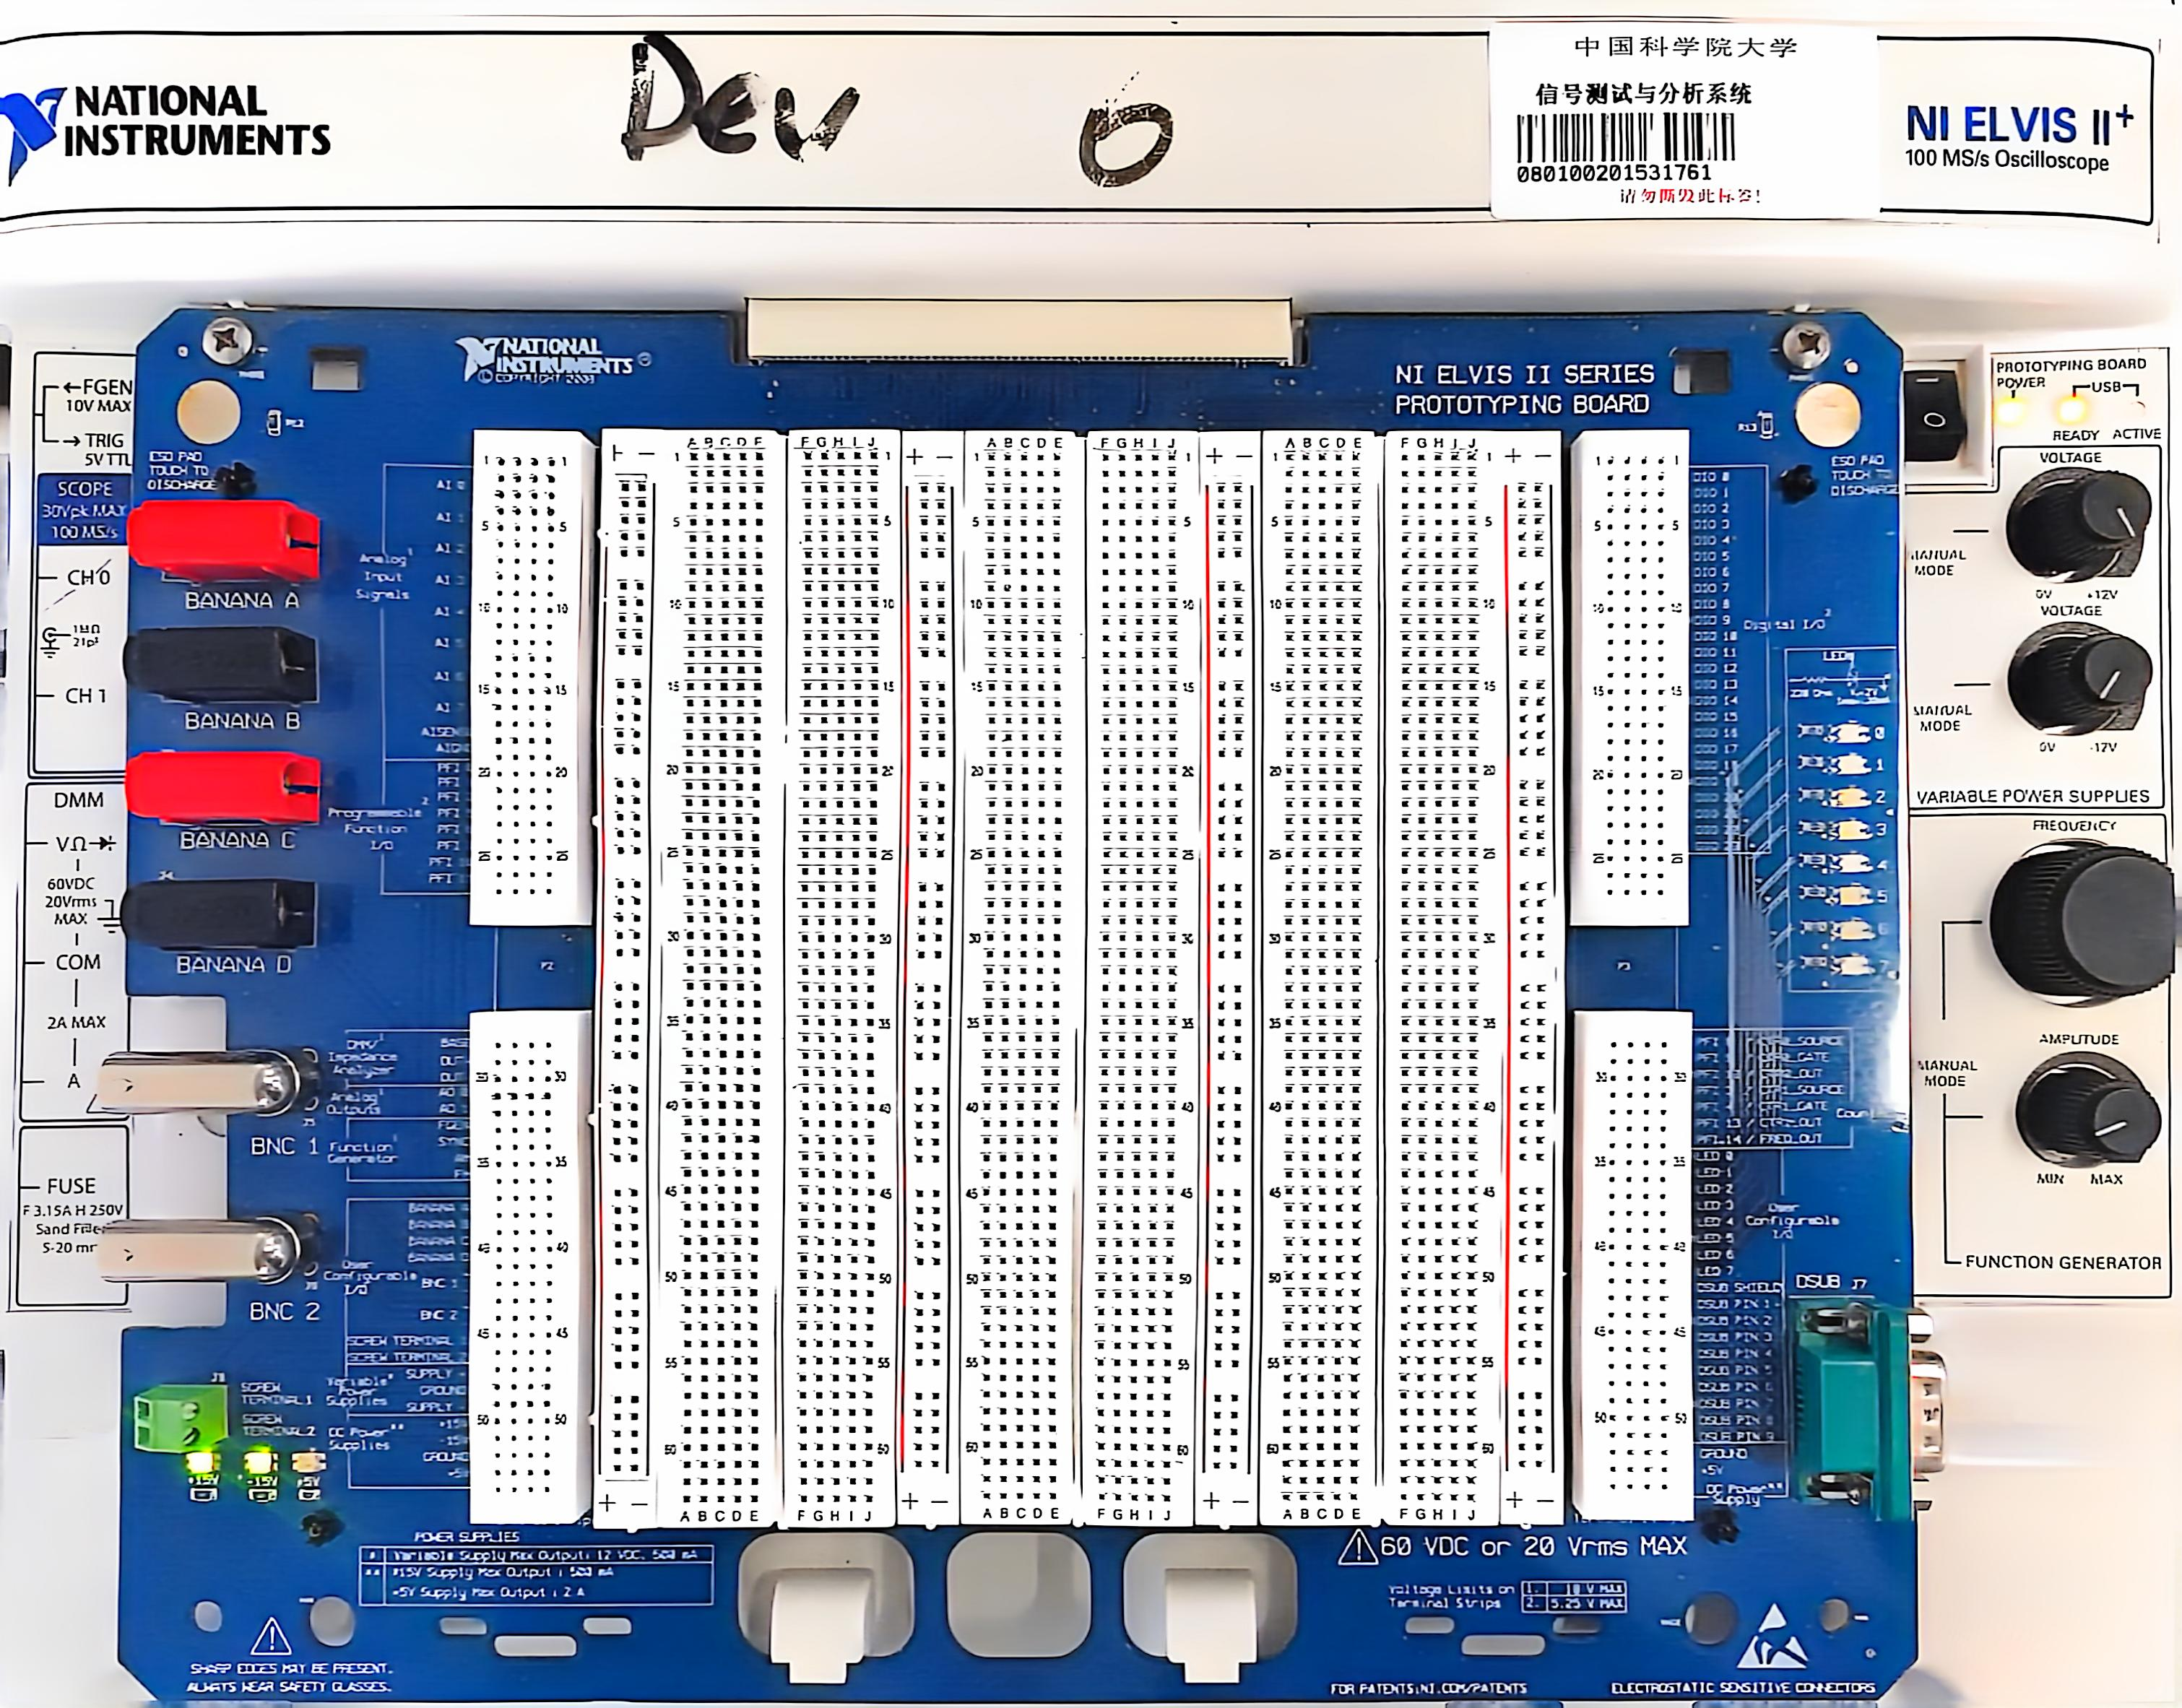
\includegraphics[height=180pt]{assets/NI ELVIS 2 和原型板实物图.jpg}
    \caption{ NI ELVIS Ⅱ 和原型板实物图 }
\end{subfigure}\hfill
\begin{subfigure}[t]{0.52\columnwidth}\centering
    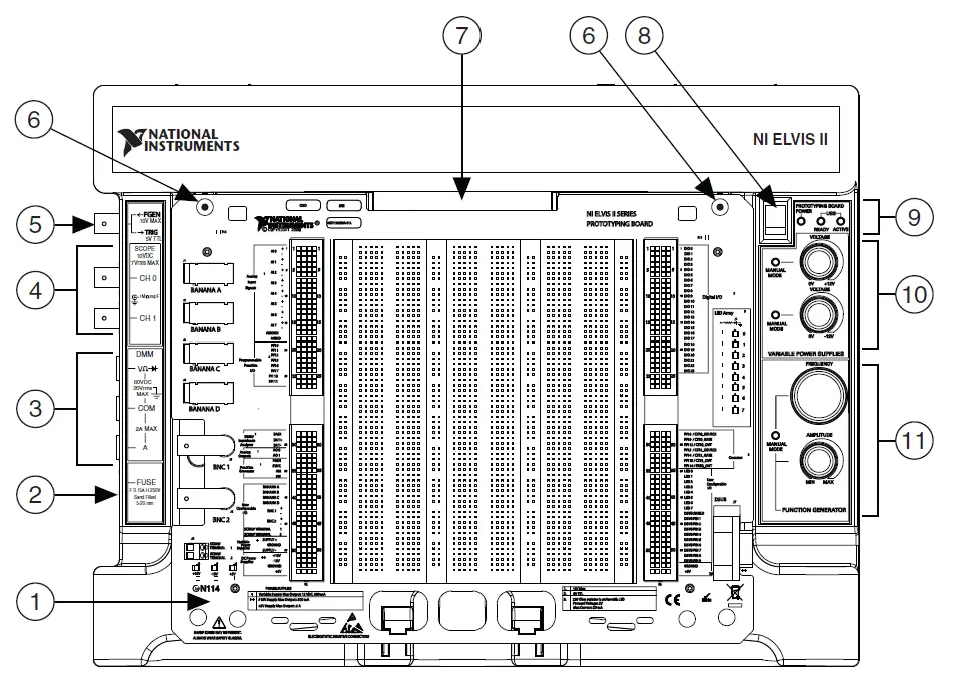
\includegraphics[height=180pt]{assets/功能说明.png}
    \caption{ NI ELVIS Ⅱ 功能说明 }
\end{subfigure}
\caption{ NI ELVIS Ⅱ }
\label{NI ELVIS Ⅱ}
\end{figure}
图 \ref{NI ELVIS Ⅱ} (a) 是 NI ELVIS Ⅱ 原型板实物图,图 \ref{NI ELVIS Ⅱ} (b) 和表 \ref{NI ELVIS Ⅱ 功能说明} 是其功能说明。
\begin{table}[H]\centering
    %\renewcommand{\arraystretch}{1.5} % 调整行间距为 1.5 倍
    %\setlength{\tabcolsep}{1.5mm} % 调整列间距
    \caption{NI ELVIS Ⅱ 功能说明}
    \label{NI ELVIS Ⅱ 功能说明}
\begin{tabular}{ll}\toprule
    1. NI ELVIS Ⅱ系列原型板 &  7. 原型板接口 \\
    2. 数字万用表保险丝 & 8. 原型板电源开关 \\
    3. 数字万用表接口 & 9. 状态灯 \\
    4. 示波器接口 & 10. 可变电源手动控制旋钮 \\
    5. 函数发生器输出/数字触发输入接口 & 11. 函数发生器手动控制旋钮 \\
    6. 原型板安装螺丝孔 &  \\
    \bottomrule
\end{tabular}
\end{table}

虚拟仪器综合实验平台ELVIS II$ ^+ $不仅集成了8路差分输入(或16路单端输入)模拟数据采集通道、24路数字I/O通道,还集成了包括示波器、数字万用表在内的多款常用仪器。同时它是开源平台,通过USB连接PC后,用户可以在LabVIEW中进行定制,使用LabVIEW Express VI和LabVIEW Signal Express的步骤对设备进行编程,实现更多更强大的功能。	

本实验旨在初步了解虚拟仪器在物理实验中的应用,故而仅需要关心模拟信号输入输出、原型板各接口间如何连通、如何在原型板上以传统电路为原型连接电路即可。

在该平台上进行实验与传统电学实验相比,能够更为轻松而简单地搭建服务于实验者目的的实验电路,同时获得的数据也更为精确,节省了人工读数、计数的时间与精力,也能一定程度上避免传统电路元件的频繁损耗。

\subsection{LabVIEW 开发平台}

本实验采用 LabVIEW(laboratory virtual instrument engineering workbench)作为用于虚拟仪器系统设计的软件开发平台。LabVIEW将计算机数据分析和显示能力与仪器驱动程序整合在一起,为针对仪器的编程提供了许多便利。同时,与其他常见的计算机高级语言相比,LabVIEW具有图形化的特点,这一点将编程过程简化为设计流程图,实验者即便没有计算机基础,也能在很短时间内的学习中掌握LabVIEW编程的基本操作与初级技巧。

用LabVIEW进行编程的集成开发环境简称VI,其包括三个部分:前面板(front panel)、程序框图(Block diagram)和图标 / 连线板。

前面板用于设置输入数值与显示输出量,相当于真实仪表的前面板,类比到常见的计算机软件中即为GUI部分(Graphical User Interface,图形用户界面)。前面板上的图标分为输入类(Controls)和显示类(Indicators),具体而言可以是开关、旋钮、图形、图表等表现形式。

程序框图则相当于仪器的内部功能结构,类似常见计算机软件中的后台进程。程序框图中的端口用于和前面板的输入对象和显示对象传递数据,节点用于实现函数与功能子程序调用,图框用于实现结构化程序控制命令,连线则代表程序执行过程中的数据流。

如ELVIS II$ ^+ $一样,LabVIEW的功能丰富而强大,而本次实验中仅聚焦于为实现实验目的的一部分即可。

\subsection{用 LabVIEW 测量伏安特性曲线}
回顾应用传统仪器测定伏安特性曲线的实验原理,图 \ref{用传统方法和虚拟仪器方法测量伏安特性曲线} (a) 给出了应用两个电压表$ U_0,U_1 $与一个标准电阻$ R_0 $来测定待测电阻$ R_1 $的大小。
\begin{equation}
    R=\frac{U_0-U_1}{U_1}\cdot R_0
\end{equation}
\begin{figure}[H]\centering
\begin{subfigure}[t]{0.5\columnwidth}\centering
    \begin{circuitikz}
        \draw (0,0)
        to[battery,l=$ \mathscr E $] (6,0)
        to[short] (6,2)
        to[european resistor,l_=$ R_0 $] (3,2)
        to[european resistor,l_=$ R_1 $] (0,2);
        \draw (3,2)
        to[short,*-] (3,1)
        to[voltmeter,-*,l_=$ U_1 $] (6,1);
        \draw (0,0)
        to[short,*-] (0,-1)
        to[voltmeter,l_=$ U_0 $] (6,-1)
        to[short,-*] (6,0);
        \draw (0,0)
        to[short] (0,2);
    \end{circuitikz}
    \caption{ 传统实验“伏伏法”测电阻伏安特性曲线电路图}
\end{subfigure}\hfill
\begin{subfigure}[t]{0.5\columnwidth}\centering
    \begin{circuitikz}
        \draw (0,-1) node[ground]{}
        to[short] (0,3)
        to[short,l=ELVIS输出端供电] (6,3)
        to[short] (6,1);
        \draw (0,1)
        to[short,*-] (0.5,1)
        to[european resistor,l=标准电阻] (3,1)
        to[european resistor,l=待测电阻] (5.5,1)
        to[short] (6,1);
        \draw (0.5,1)
        to[short,*-] (0.5,2)
        to[short,l=测总电压] (5.5,2)
        to[short,-*] (5.5,1);
        \draw (0.5,1)
        to[short] (0.5,0)
        to[short,l_=测电压算电流] (3,0)
        to[short,-*] (3,1);
    \end{circuitikz}
    \caption{用虚拟仪器测量伏安特性原理图}
\end{subfigure}
\caption{用传统方法和虚拟仪器方法测量伏安特性曲线}
\label{用传统方法和虚拟仪器方法测量伏安特性曲线}
\end{figure}
由串联电路的分压原理可知,用总电压$ U_0 $减去标准电阻上的电压$ U_1 $即得到待测电阻上的电压;根据欧姆定律可知,用标准电阻上的电压$ U_1 $除以标准电阻阻值$ R_0 $即可得到电路中的电流$ I $。最后再由欧姆定律即可求得待测电阻的阻值。

当然,为进一步渐消实验误差,还需多次改变电源的电动势$ \mathscr E $以获得多组实验数据。如需测定二极管的伏安特性曲线,则除将待测电阻替换为二极管外,还需根据二极管正反接情况调整电源、电压表的正负极接线。

应用虚拟仪器测定伏安特性的电路见图 \ref{用传统方法和虚拟仪器方法测量伏安特性曲线} (b)。与传统利用电源电动势为整个电路供电不同,本实验中利用一个模拟输出通道为整个测量电路供电,同时利用两个模拟输入通道取代电压表,分别测量总电压与标准电阻上的电压。

求得阻值的方式与传统仪器实验并无不同,而读数、计算、线性拟合这些工作虚拟仪器实验中都交由计算机来完成,节省了时间与精力。此外,虚拟仪器可由程序控制总电压从$ 0\,\mathrm V $开始逐渐增加到指定电压,不需要频繁手工设置相应电动势的电源。在测定二极管伏安特性曲线时,切换正反接时也无需重新接线,仅将电压递增步长调整为负值即可。

% ---------------------------------------------------- 

\section{实验内容与步骤}
\subsection{熟悉开发环境}
通过各种方式之一启动LabVIEW 2014后,新建VI项目即可得到新项目的前面板与程序框图。通过在这两个窗口间切换、探索,我们不难初步了解如何快速切换到另一个窗口、如何添加调整各种控件、控件调整时两个窗口间的同步变化、丰富的右键快捷菜单,学习标签工具、定位工具、连线工具乃至各种快捷键。

LabVIEW 开发环境如图 \ref{LabVIEW 开发环境} 所示,左侧是前面板窗口,右侧是程序框图窗口。

\begin{figure}[H]\centering
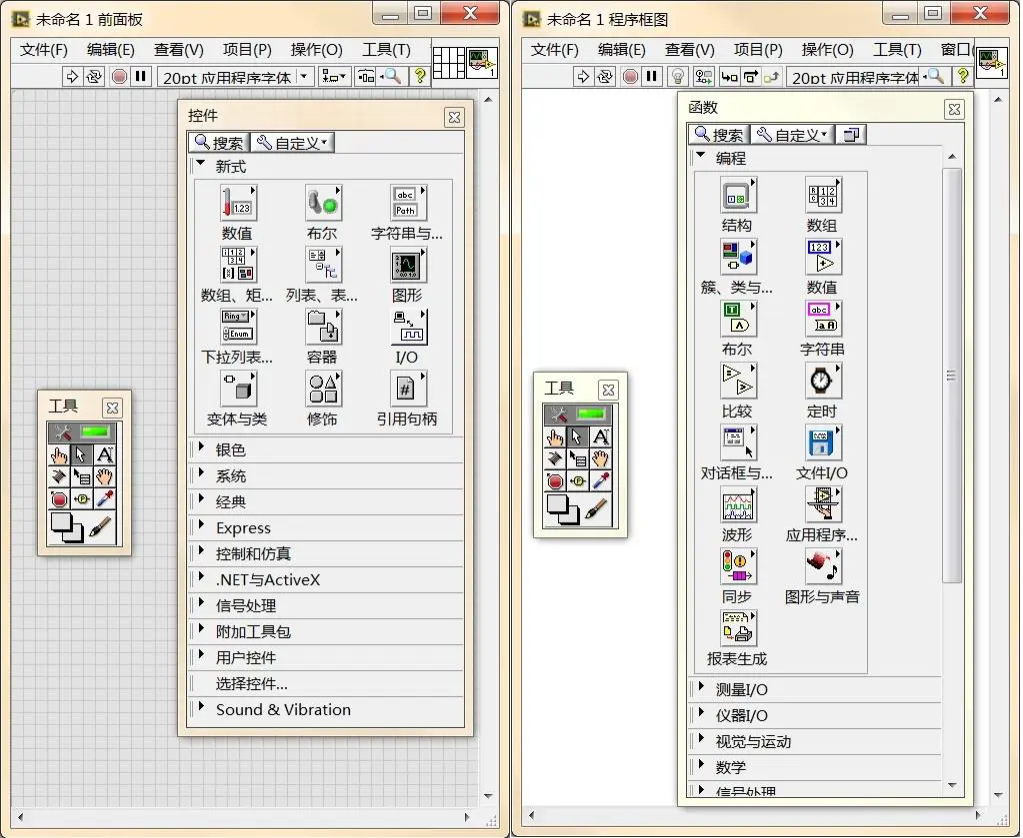
\includegraphics[width=0.75\columnwidth]{assets/LabVIEW开发环境.png}
\caption{LabVIEW 开发环境}\label{LabVIEW 开发环境}
\end{figure}

\subsection{模拟温度测量}
那么可以利用计算机程序由电压值来计算温度值,同时我们希望程序中可以用开关来使温度单位在摄氏度与华氏度间切换。为使实验简单,采用一个输入控件来替代数据采集卡对传感器的测量结果。不妨假设传感器的输出电压与温度成正比,且传感器输出 0.8 V 时,对应的华氏温度为 80 $^\circ$F,则将测得的电压值乘 100 即可得到华氏温度值。如需显示摄氏温度值,则再将其转换为摄氏温度即可。程序搭建完毕后,效果如图 \ref{模拟温度测量} 所示。
\begin{figure}[H]\centering
\begin{subfigure}[t]{0.52\columnwidth}\centering
    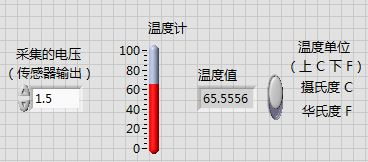
\includegraphics[height=105pt]{assets/模拟温度测量 面板_2.JPG}
    \caption{ 前面板 }
\end{subfigure}\hfill
\begin{subfigure}[t]{0.48\columnwidth}\centering
    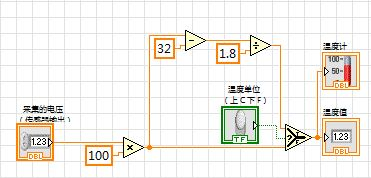
\includegraphics[height=105pt]{assets/模拟温度测量 框图.JPG}
    \caption{ 程序框图 }
\end{subfigure}
\caption{ 模拟温度测量 }
\label{模拟温度测量}
\end{figure}

\noindent 具体实验步骤为:
\begin{enumerate}
\item 新建VI项目,在前面板中,放入温度计、垂直滑动杆开关、数值显示控件、数值输入控件,并利用标签工具修改其名称以表示所需的含义。
\item 在程序框图中,在函数选板中找到乘法、减法、除法、比较函数,将其与相应的图标通过连线工具连接起来,并在需要的地方创建数值常量。整个程序创建完毕后,最后整理图标位置与连线,使得程序框图更为美观。
\item 运行程序:选择前面板窗口,点击连续运行按钮使得程序运行于连续运行模式,改变“采集的电压”控件输入值和温度值单位,观察程序运行情况。再次点击连续运行按钮即可停止程序运行。
\item 保存该VI项目,关闭程序。
\end{enumerate}


\subsection{电压输出采集}
此实验中,除了进一步温习上一个实验中在前面板、程序框图上的设计操作,还开始使用了原型板,了解了如何简单地将原型板与计算机程序进行交互。计算机程序指示原型板在模拟输出端输出指定大小的电压,通过连线后使得原型板上模拟输入端与之等压,再将模拟输入端读入的数据呈递给计算机程序。此外,再LabVIEW程序设计上还进一步了解了While循环结构的设计方式。搭建程序并连接实物电路,最终效果如图 \ref{电压输出与采集} 所示。

\noindent 具体实验步骤为:
\begin{enumerate}
\item 新建VI项目,在程序框图中创建虚拟通道,将其类型设置为模拟输出电压。将“DAQmx开始任务”、“DAQmx写入”和“DAQmx清除任务”三个节点放入程序框图,并将其连接,在“DAQmx写入”的图标数据输入端创建输入控件。创建一个While循环结构,使得每等待100\,ms执行一次循环结构内部分,直至在前面板按下停止按钮。
\item 编写电压采集程序,在程序框图中创建虚拟输入电压通道,以类似的方式构建任务链与While循环,不同之处在于此处不采用“DAQmx写入”控件而是“DAQmx读取”控件,其连接输出控件而非输入控件;While循环中每100\,ms所执行的操作并非重新读取输出电压而是重新输出采集电压数据。
\item 通过USB线连接PC与原型板,打开ELVIS电源与原型板电源,在前面板上设置输出通道为Dev7/ao0(Dev后编号视实际连接结果而定),输入通道为Dev7/ai0。在原型板上用原型板连接模拟输出的“AO 0”端和模拟输入的“AI $ 0+ $”端,将“AI $ 0- $”端与接地端“AIGND”用导线连接。在前面板窗口运行VI程序,不断改变输出电压,观察测量电压是否与输出电压一致,也可点击停止按钮观察程序运行情况。
\item 停止程序运行,保存VI项目,关闭程序。
\end{enumerate}

\begin{figure}[H]\centering
    \begin{minipage}[t]{0.48\textwidth}
        \centering
        \begin{subfigure}[b]{\textwidth}
            \centering
            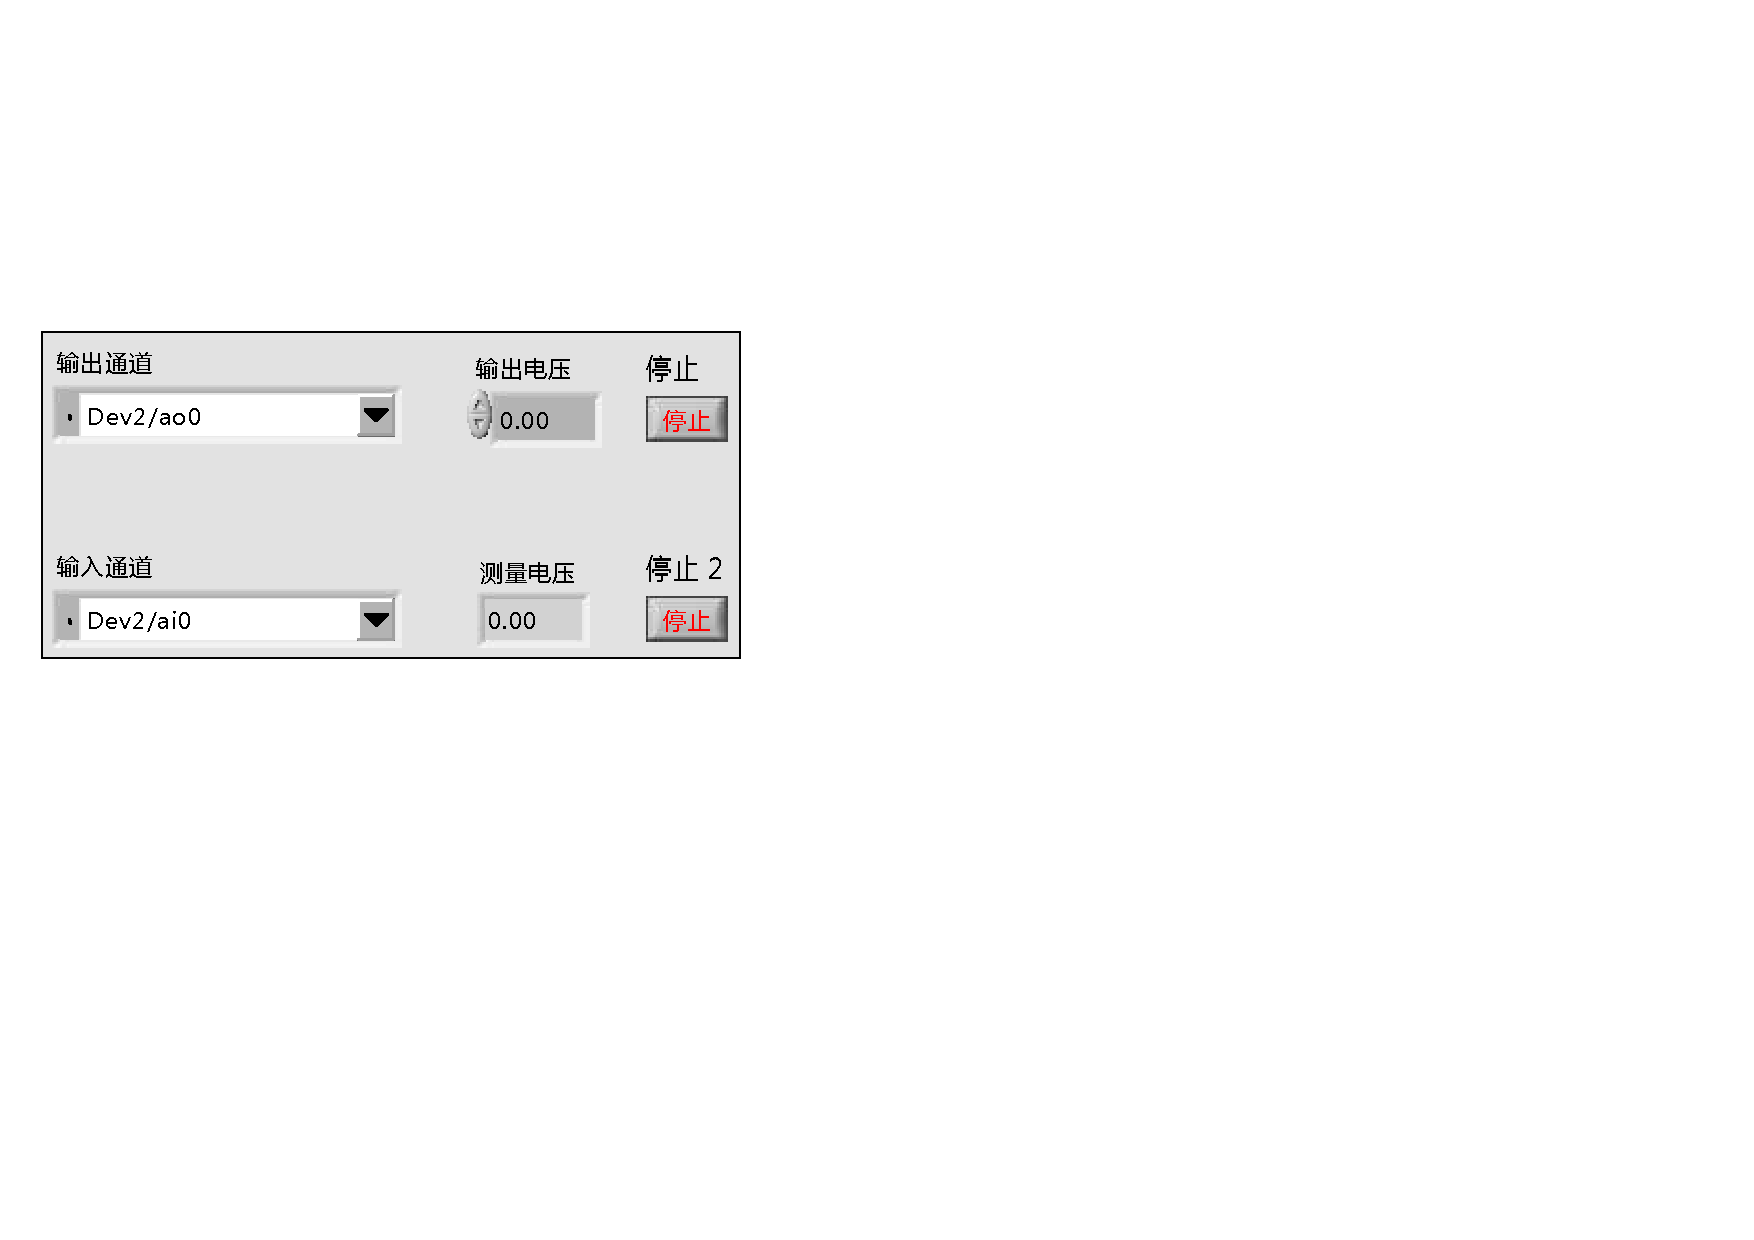
\includegraphics[height=110pt]{assets/电压输出采集__面板.pdf}
            \caption{前面板}
        \end{subfigure}
        \vfill
        \begin{subfigure}[b]{\textwidth}
            \centering
            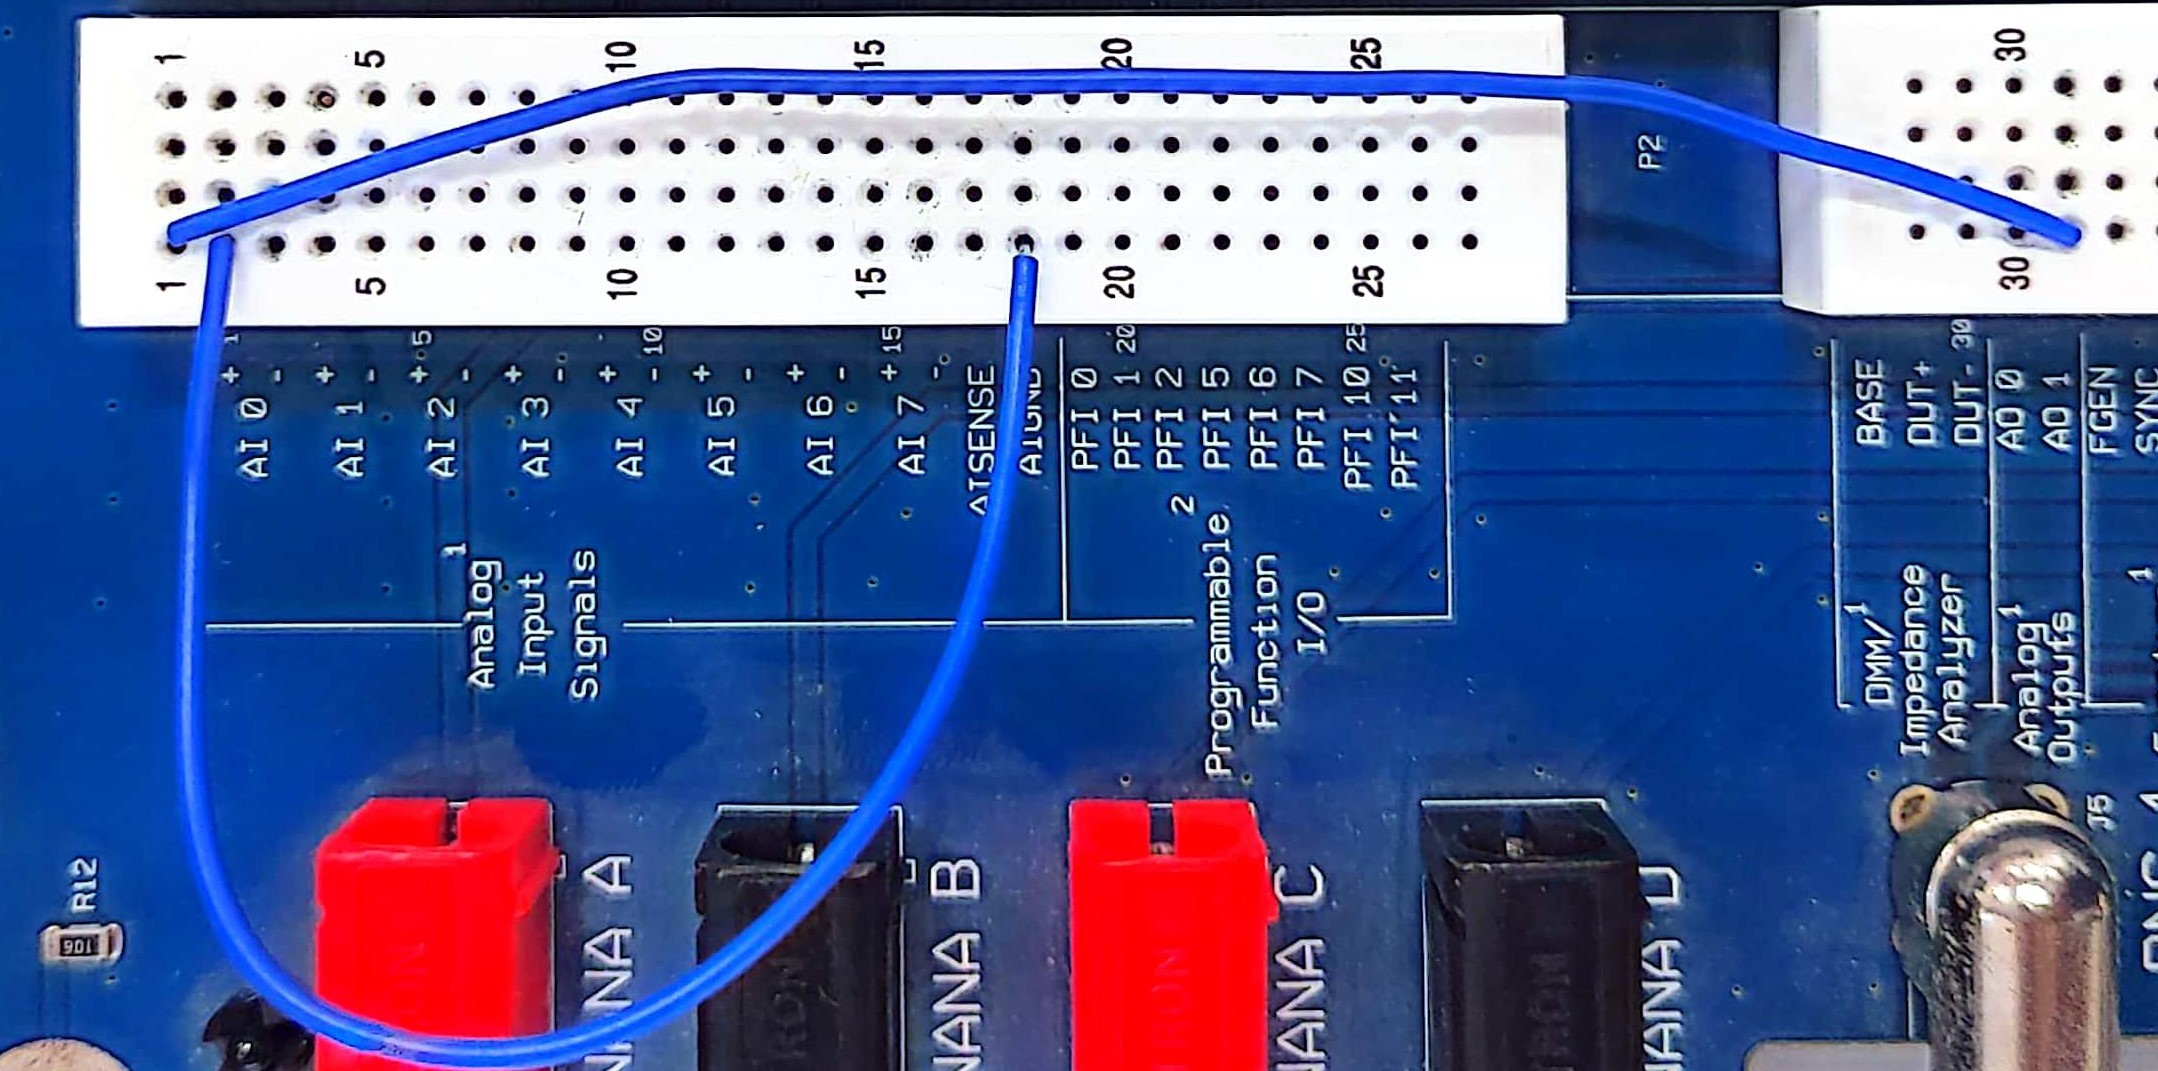
\includegraphics[height=110pt]{assets/电压输出与采集.jpg}
            \caption{程序框图}
        \end{subfigure}
    \end{minipage}
    \hfill
    \begin{minipage}[H]{0.48\textwidth}
        \centering
        \begin{subfigure}[b]{\textwidth}
            \centering
            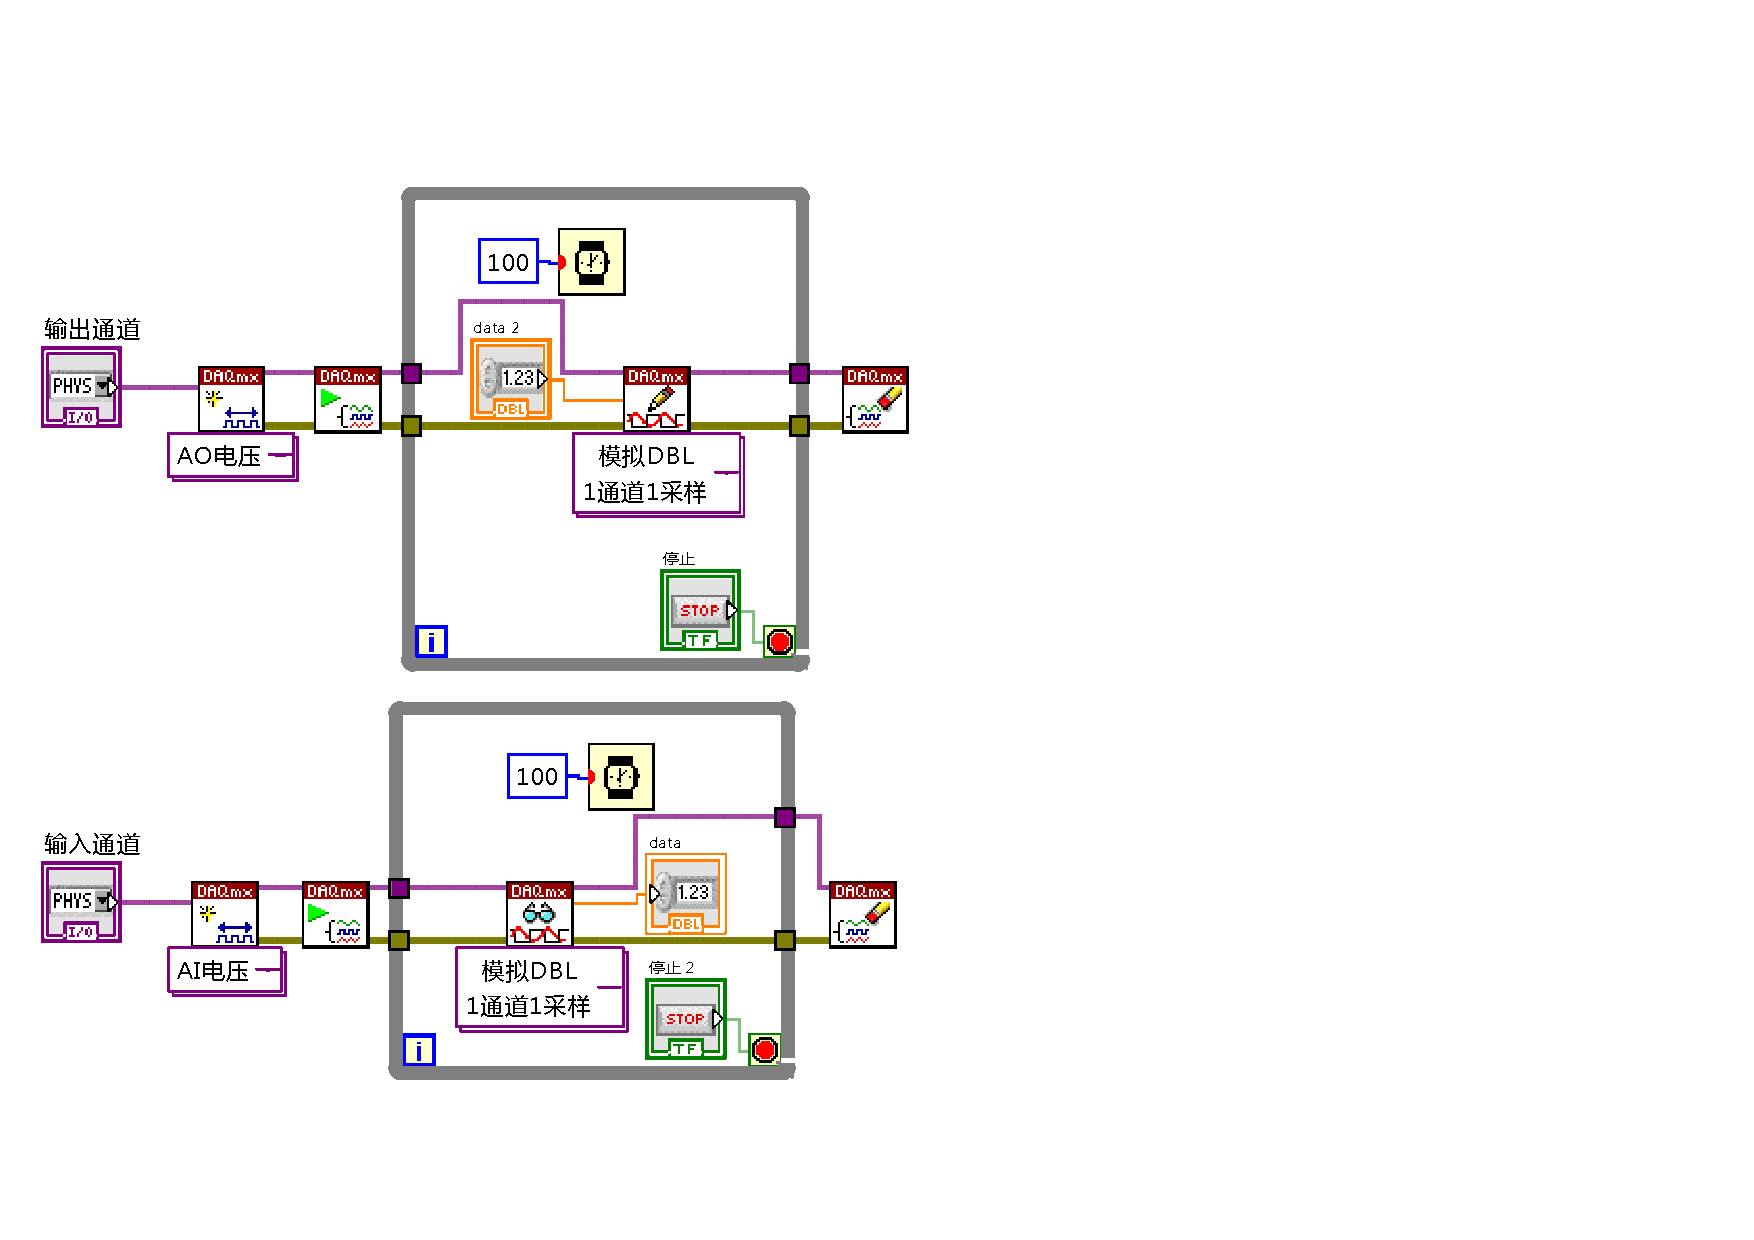
\includegraphics[height=240pt]{assets/电压输出采集__框图.pdf}
            \caption{电路连接方式}
        \end{subfigure}
    \end{minipage}
    \caption{电压输出与采集}
    \label{电压输出与采集}
\end{figure}



\subsection{测量伏安曲线}
在此小节,我们编写一个较前两实验更为复杂,同时也为我们所熟知的实验程序,先对两个不同的待测电阻进行阻值测定与伏安特性曲线绘制,然后利用虚拟仪器设置反向电压的便利来测定二极管的正反向的伏安特性曲线。搭建完成的前面板如图 \ref{测量伏安特性曲线的前面板} 所示,程序框图如图 \ref{测量伏安特性曲线的程序框图} 所示。


\begin{figure}[H]\centering
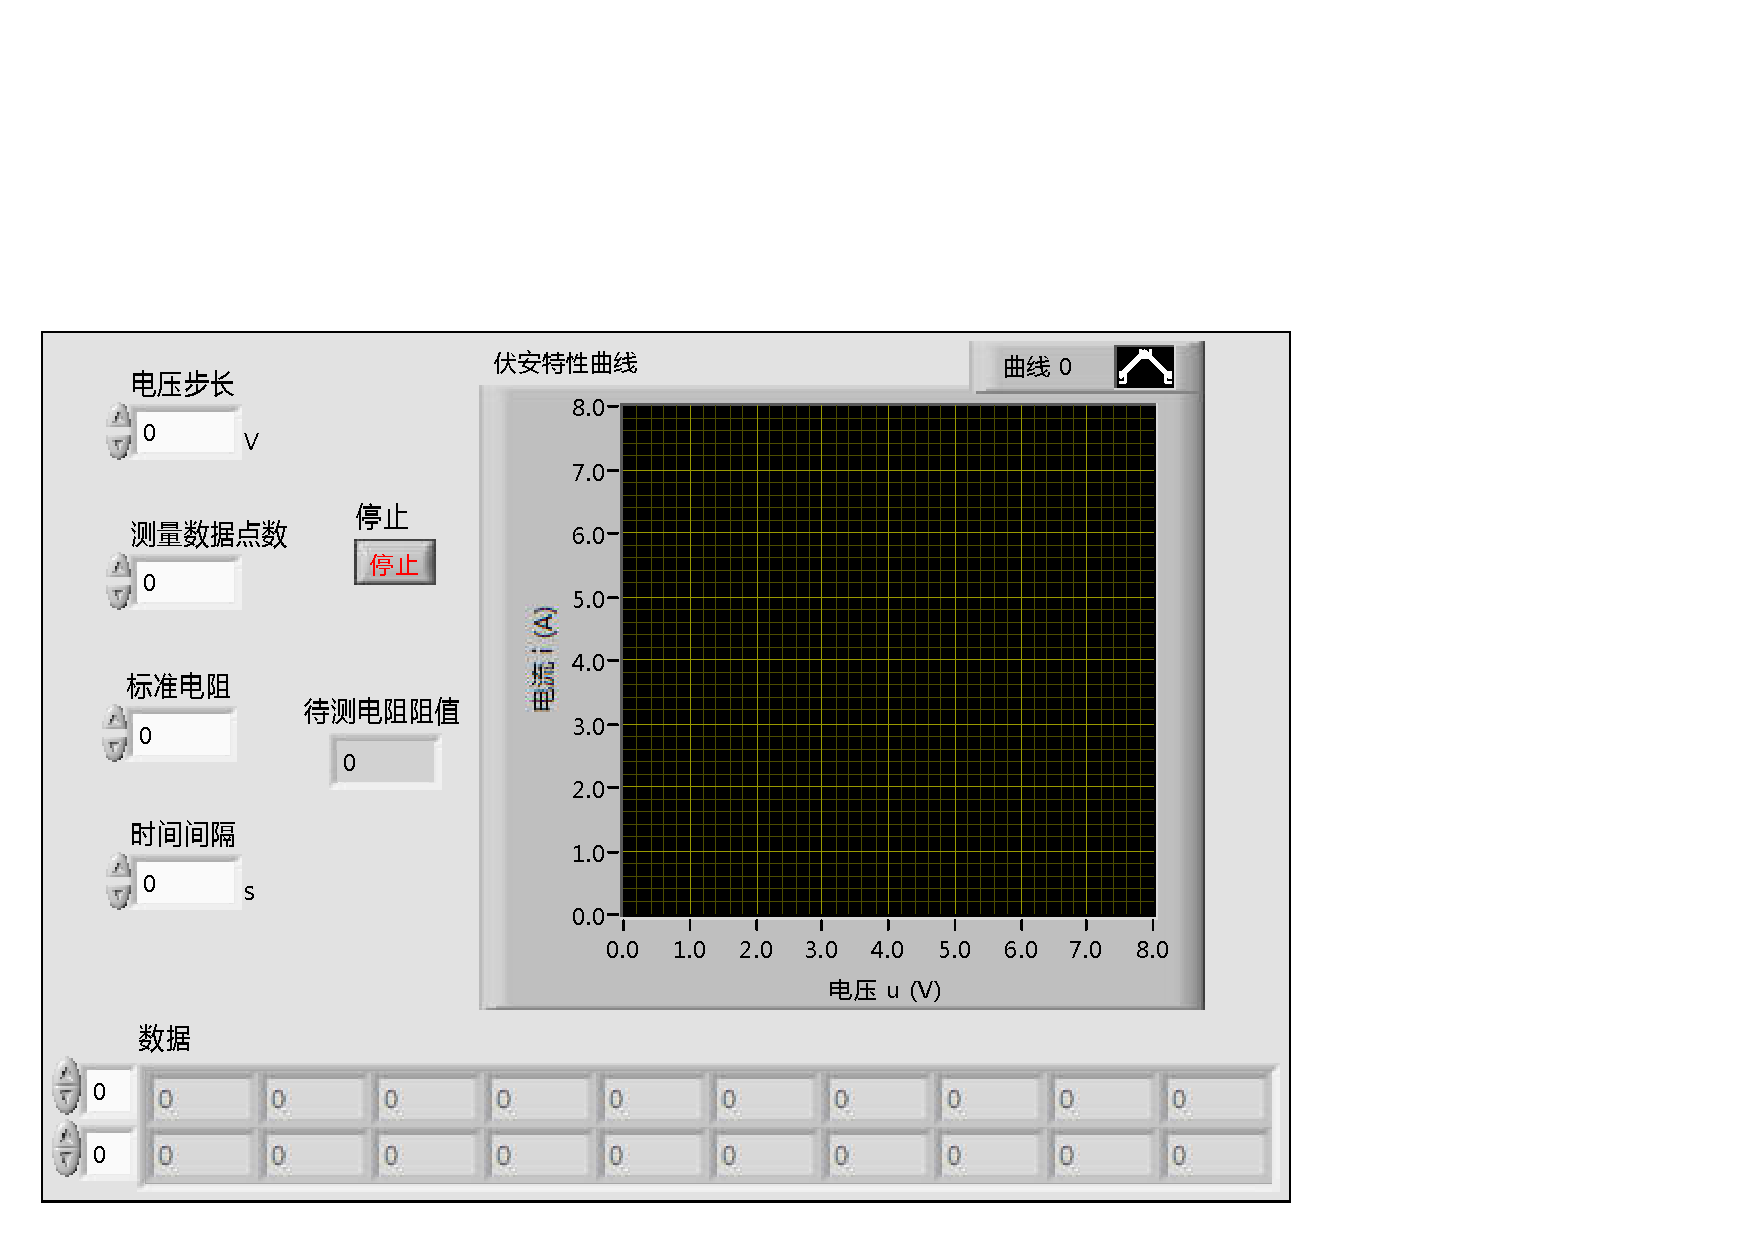
\includegraphics[width=0.7\columnwidth]{assets/测量伏安曲线__面板.pdf}
\caption{测量伏安特性曲线的前面板}\label{测量伏安特性曲线的前面板}
\end{figure}
\begin{figure}[H]\centering
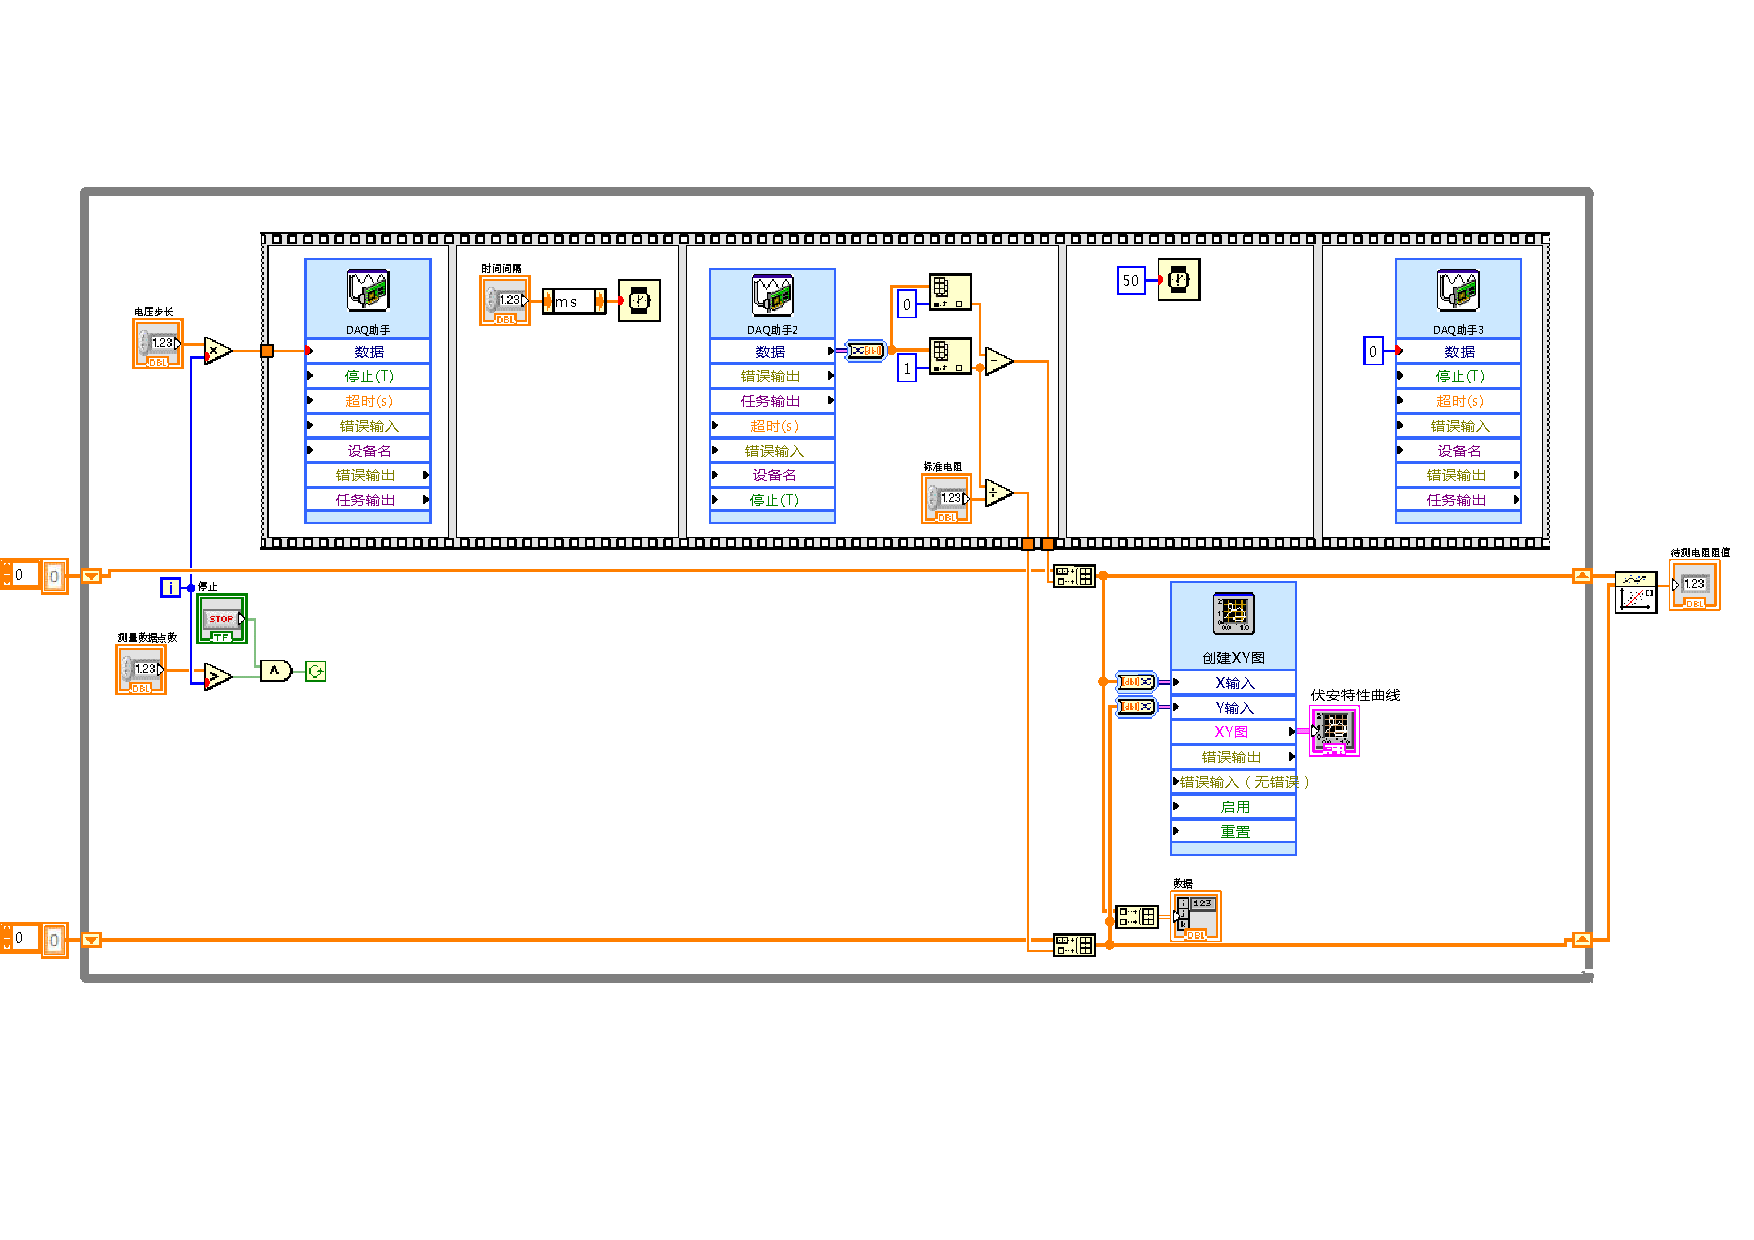
\includegraphics[width=\columnwidth]{assets/测量伏安曲线__框图.pdf}
\caption{测量伏安特性曲线的程序框图}\label{测量伏安特性曲线的程序框图}
\end{figure}

\noindent 具体实验步骤如下:
\begin{enumerate}
\item 编写前面板:在前面板上放上 Express XY 图用于显示电压--电流图。放入四个数值型输入控件,分别用于输入“输出电压步长”、“测量数据点数”、“标准电阻”、“时间间隔”四个参数,并规定时间间隔与输入电压步长的单位。放入一个数值型显示控件用于显示电阻测量值,放入一个二维数组显示控件用于显示测量的电压和电流。最后放入一个开关用于控制程序进程。
\item 编写程序框图:放入一个 5 帧的顺序结构,第0帧用于让ELVIS输出电压,第1帧让程序等待100\,ms至电路稳定,第2帧用于让ELVIS采集总电压与标准电阻上的电压,第3帧再次让程序等待100\,ms以减少对数据测量过程的影响,第4帧令顺序结构结束时电压输出为0。这样的顺序结构实现了测量一次的过程,要逐渐改变电压值来测量电阻的值,还需加入一个While循环结构,使得While循环及其中的顺序结构在执行次数i不大于测量数据点数时循环执行。通过一个“创建数组”来显示测量数据,将电压、电流数组分别与“创建XY图”的X、Y输入相连。为求得电阻值,需在循环外放入一个“线性拟合”节点,用于拟合并显示电阻值。
\item 正根据实验原理部分中给出的原理电路图与上一步 DAQ 助手设置的输入输出端口,并在实际原型板上正确连接实验电路。
\item 在前面板上设置好参数,运行程序以测量两个待测元件的伏安曲线,分析实验数据与结果。
\item 另外,还可以改变“电压步长”的正负来给待测元件两端加上正反向电压,由此测定并绘制较完整的伏安特性曲线。
\end{enumerate}

需要测量的四个元件分别是 $51 \ \Omega$ 电阻、$1 \ \kO$ 电阻、整流二极管和发光二极管,如图 \ref{四个待测元件} 所示,测量结果见下一节“实验结果与数据处理”。

\begin{figure}[H]\centering
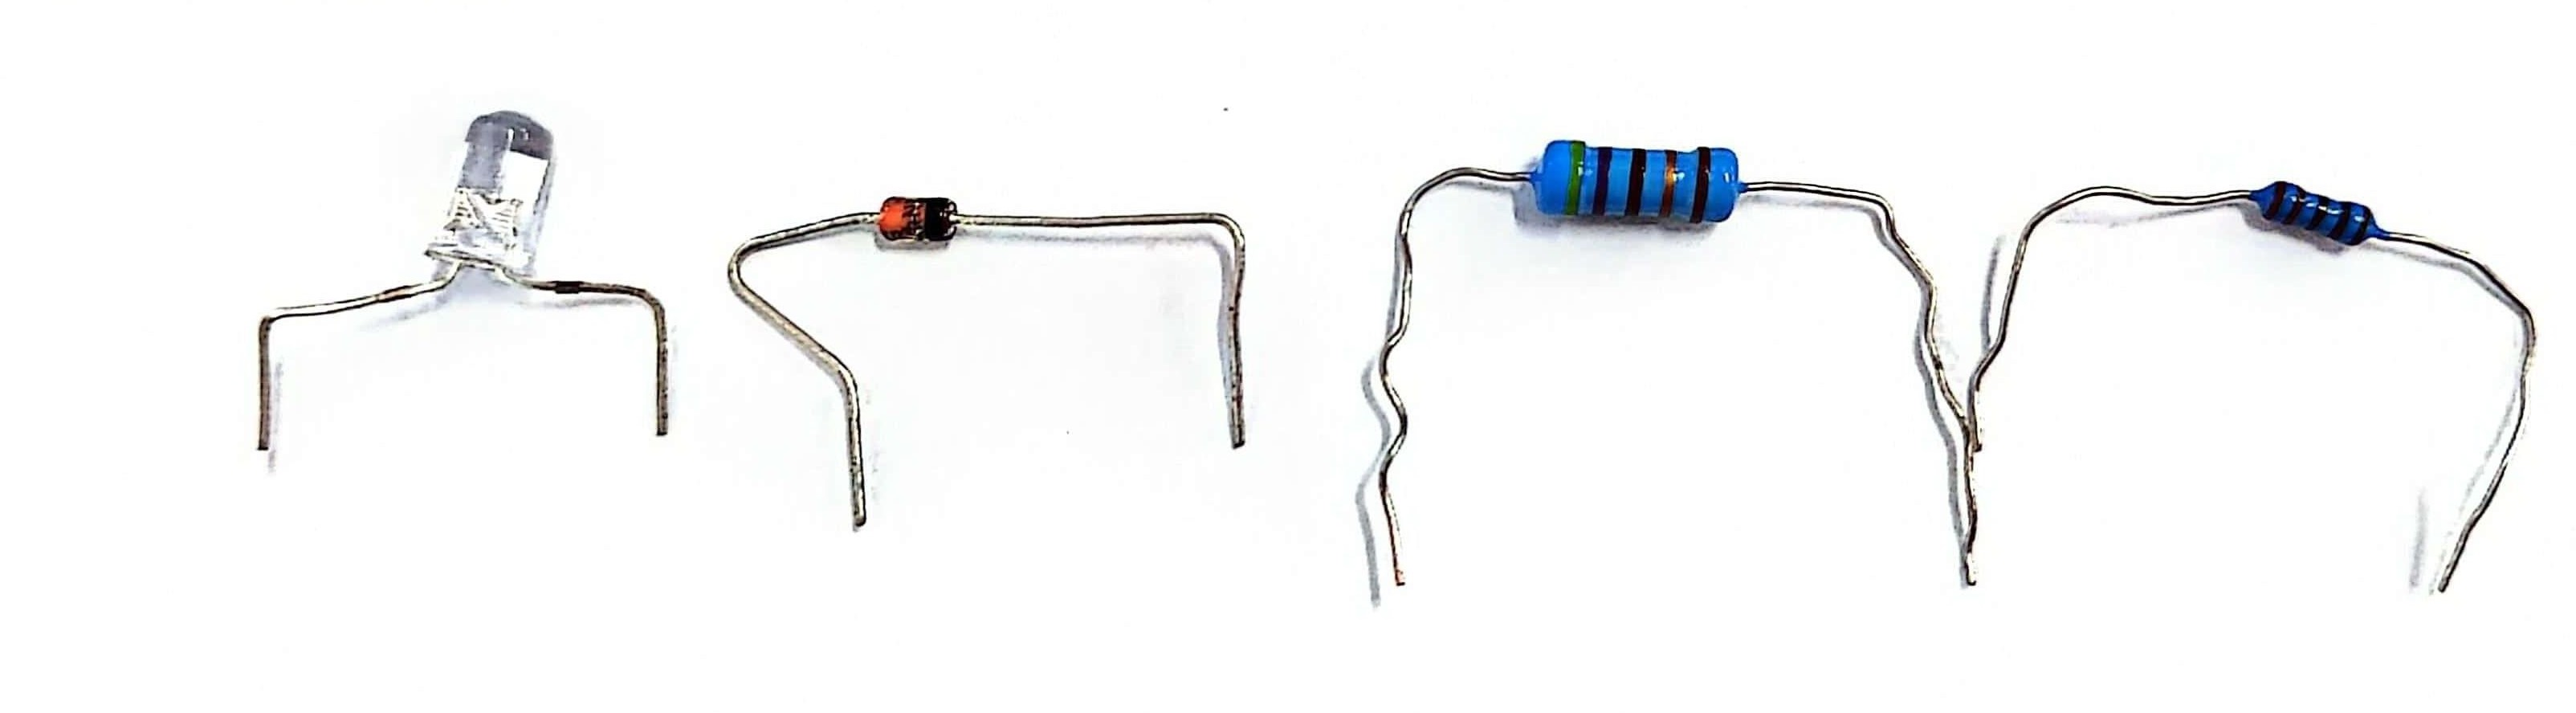
\includegraphics[height=125pt]{assets/四个待测元件.jpg}
\caption{发光二极管、整流二极管、$51 \ \Omega$ 电阻、$1.00 \ \kO$ 电阻(从左至右)}\label{四个待测元件}
\end{figure}

\newpage
\section{实验结果与数据处理}

\subsection{$51 \ \Omega$ 电阻}
待测元件是标定值为 $51 \ \Omega$ 的线性电阻,前面板参数设置和电路连接方式见图 \ref{测量51欧电阻的伏安曲线},所得 $u$-$i$ 数据如表 \ref{51欧电阻伏安数据} 所示。

\begin{figure}[H]\centering
\begin{subfigure}[b]{0.45\columnwidth}\centering
    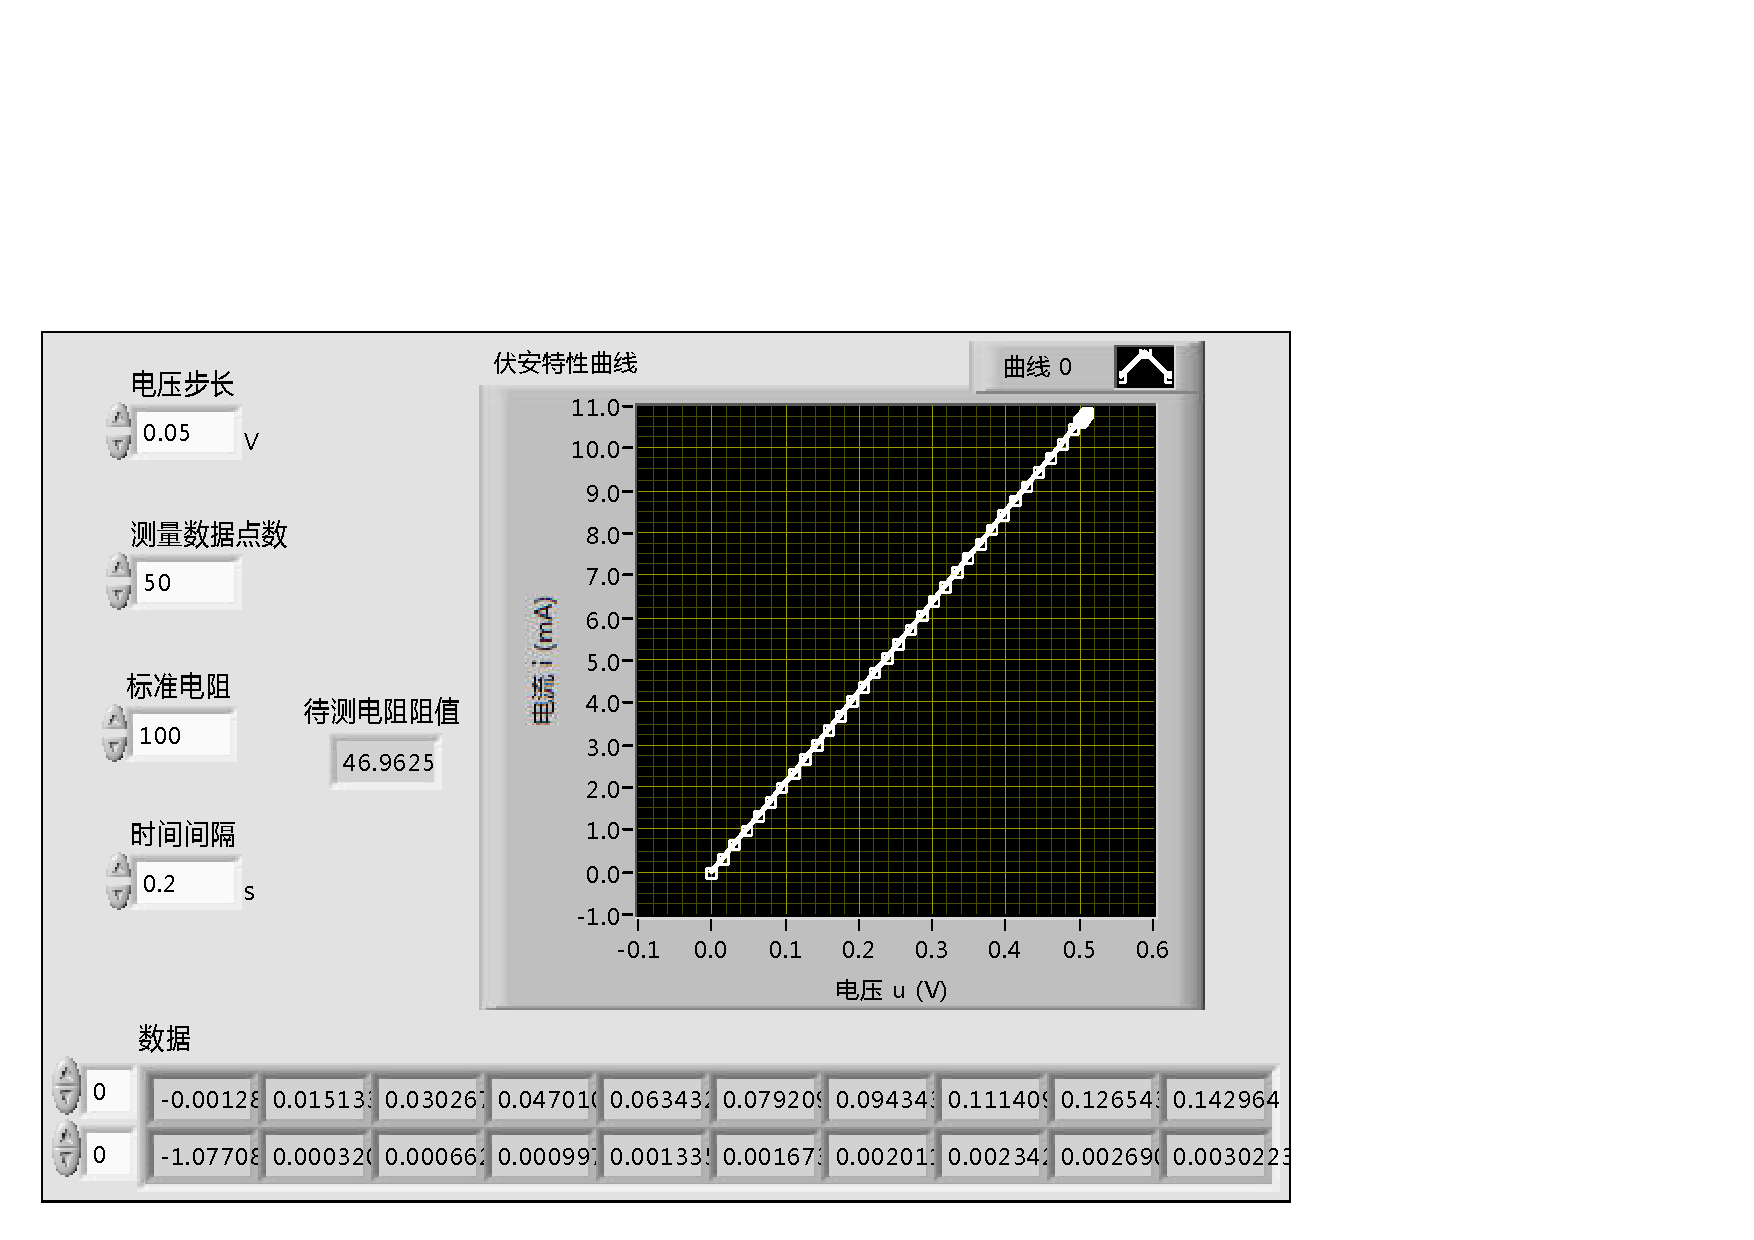
\includegraphics[height=150pt]{assets/测量伏安曲线__50欧电阻.pdf}
    \caption{前面板}
\end{subfigure}\hfill
\begin{subfigure}[b]{0.55\columnwidth}\centering
    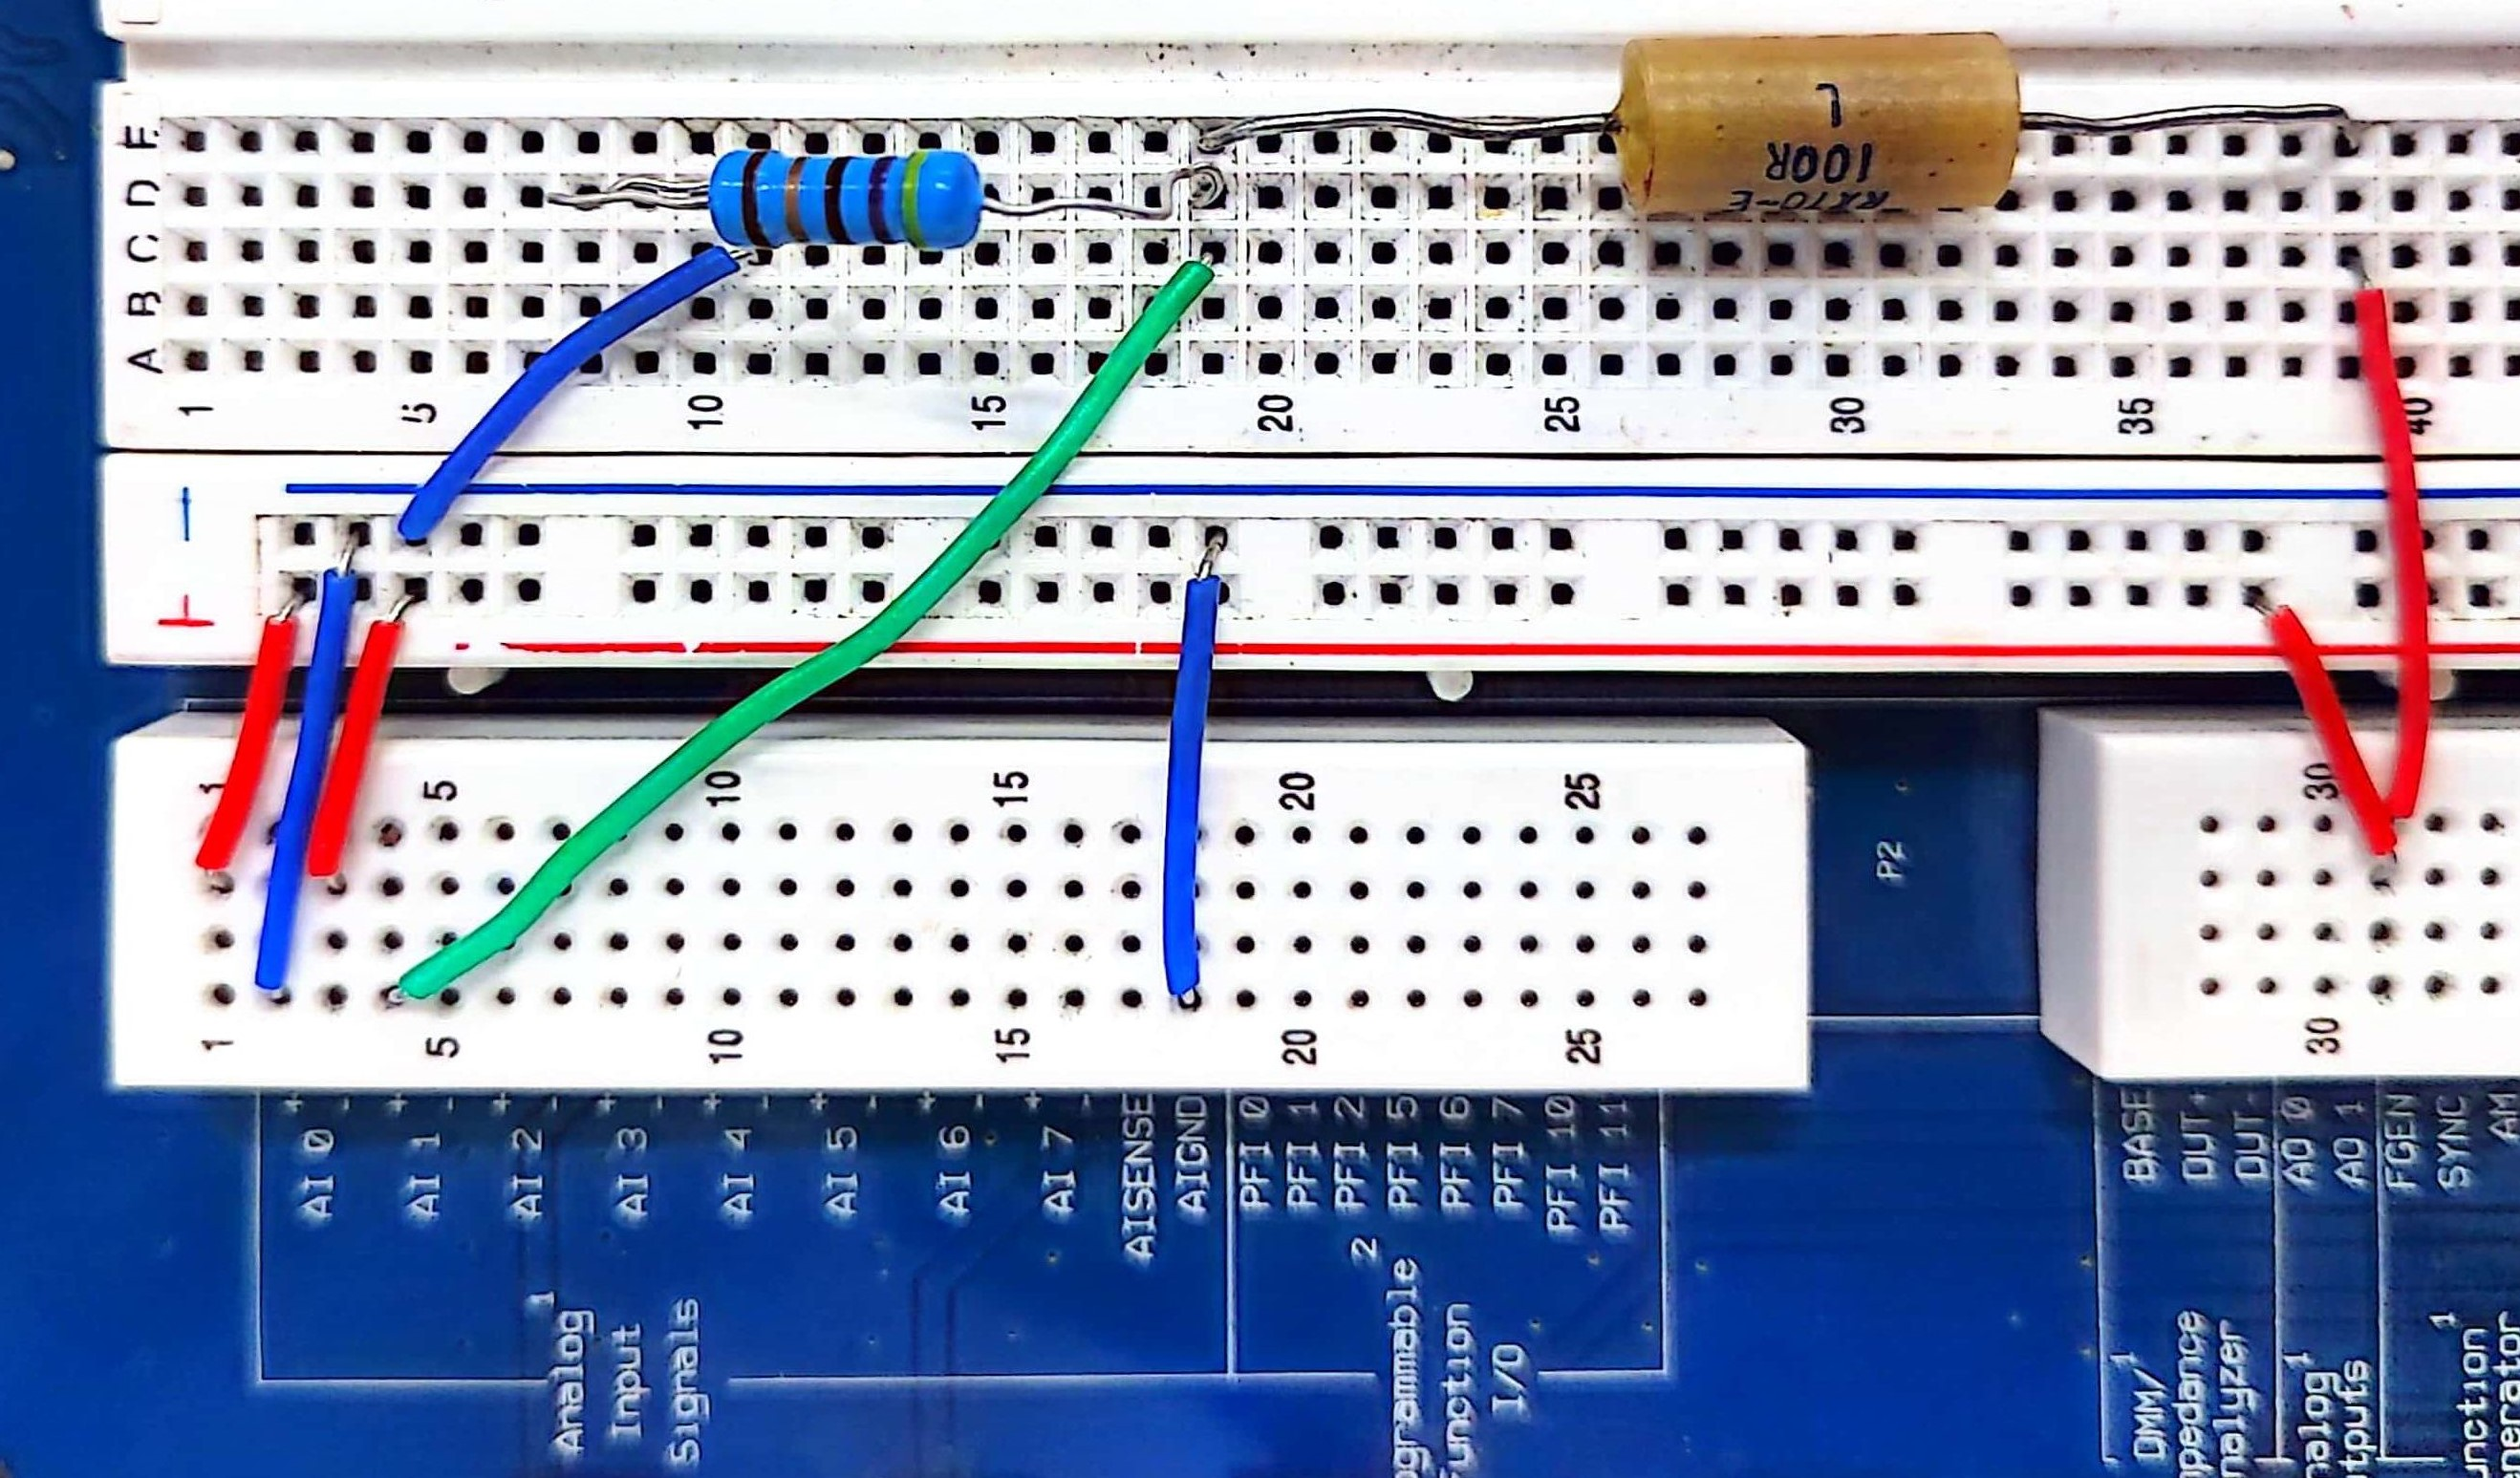
\includegraphics[height=150pt]{assets/测量伏安曲线__50欧电阻.jpg}
    \caption{实际电路连接}
\end{subfigure}
\caption{测量 $51 \ \Omega$ 电阻的伏安曲线}
\label{测量51欧电阻的伏安曲线}
\end{figure}


\begin{table}[H]\centering
%\renewcommand{\arraystretch}{1.5} % 调整行间距为 1.5 倍
%\setlength{\tabcolsep}{1.5mm} % 调整列间距
\caption{$51 \ \Omega $ 电阻的伏安数据}
\label{51欧电阻伏安数据}
\begin{tabular}{|ll|ll|ll|}
    \hline
    电压 (V)  & 电流 (A)   & 电压 (V)  & 电流 (A)   &电压 (V)  & 电流 (A) \\ \hline
    -0.00128796 & -0.00001077   & 0.253085 & 0.00539224 & 0.506816 & 0.0108017  \\ 
    0.0151336   & 0.00032088  & 0.269829 & 0.00573356 & 0.509392 & 0.0108468  \\
    0.0302672   & 0.000662191 & 0.285607 & 0.00606521 & 0.507138 & 0.010792   \\
    0.0470107   & 0.000997062 & 0.301384 & 0.00640974 & 0.50585  & 0.0107566  \\
    0.0634323   & 0.00133515  & 0.316518 & 0.00674461 & 0.504562 & 0.0107309  \\
    0.0792099   & 0.00167324  & 0.33294  & 0.00708592 & 0.503596 & 0.0107083  \\
    0.0943435   & 0.00201133  & 0.347751 & 0.00742723 & 0.501986 & 0.0106987  \\
    0.111409    & 0.00234299  & 0.365461 & 0.00775566 & 0.502308 & 0.0106826  \\
    0.126543    & 0.00269074  & 0.380273 & 0.00809698 & 0.50263  & 0.0106697  \\
    0.142964    & 0.00302239  & 0.39605  & 0.00844151 & 0.500376 & 0.0106697  \\
    0.158098    & 0.0033637   & 0.411506 & 0.00878282 & 0.500698 & 0.01066    \\
    0.174519    & 0.00369857  & 0.427606 & 0.00911125 & 0.500698 & 0.0106536  \\
    0.189975    & 0.0040431   & 0.443383 & 0.00944934 & 0.499732 & 0.0106504  \\
    0.205753    & 0.00437797  & 0.460127 & 0.00978421 & 0.500376 & 0.0106407  \\
    0.220886    & 0.0047225   & 0.476227 & 0.0101223  & 0.49941  & 0.0106472  \\
    0.237952    & 0.00505415  & 0.491038 & 0.0104701  & 0.500376 & 0.0106311  \\
    \hline
\end{tabular}
\end{table}

由 LabVIEW 程序中的线性拟合(前面板上的结果),可得电阻的测量值为 $R = 46.9625\ \Omega$。我们在 Matlab 中用最小二乘法对函数 $i = \frac{1}{R}u$ 进行拟合,得到 $R = 46.9808 \ \Omega$,两者结果基本吻合。

\newpage
\subsection{$1\ \kO$ 电阻}

待测元件是标定值为 $1 \kO$ 的线性电阻,前面板参数设置和电路连接方式见图 \ref{测量1K欧电阻的伏安曲线},所得 $u$-$i$ 数据如表 \ref{1K欧电阻伏安数据} 所示。

\begin{figure}[H]\centering
    \begin{subfigure}[b]{0.45\columnwidth}\centering
        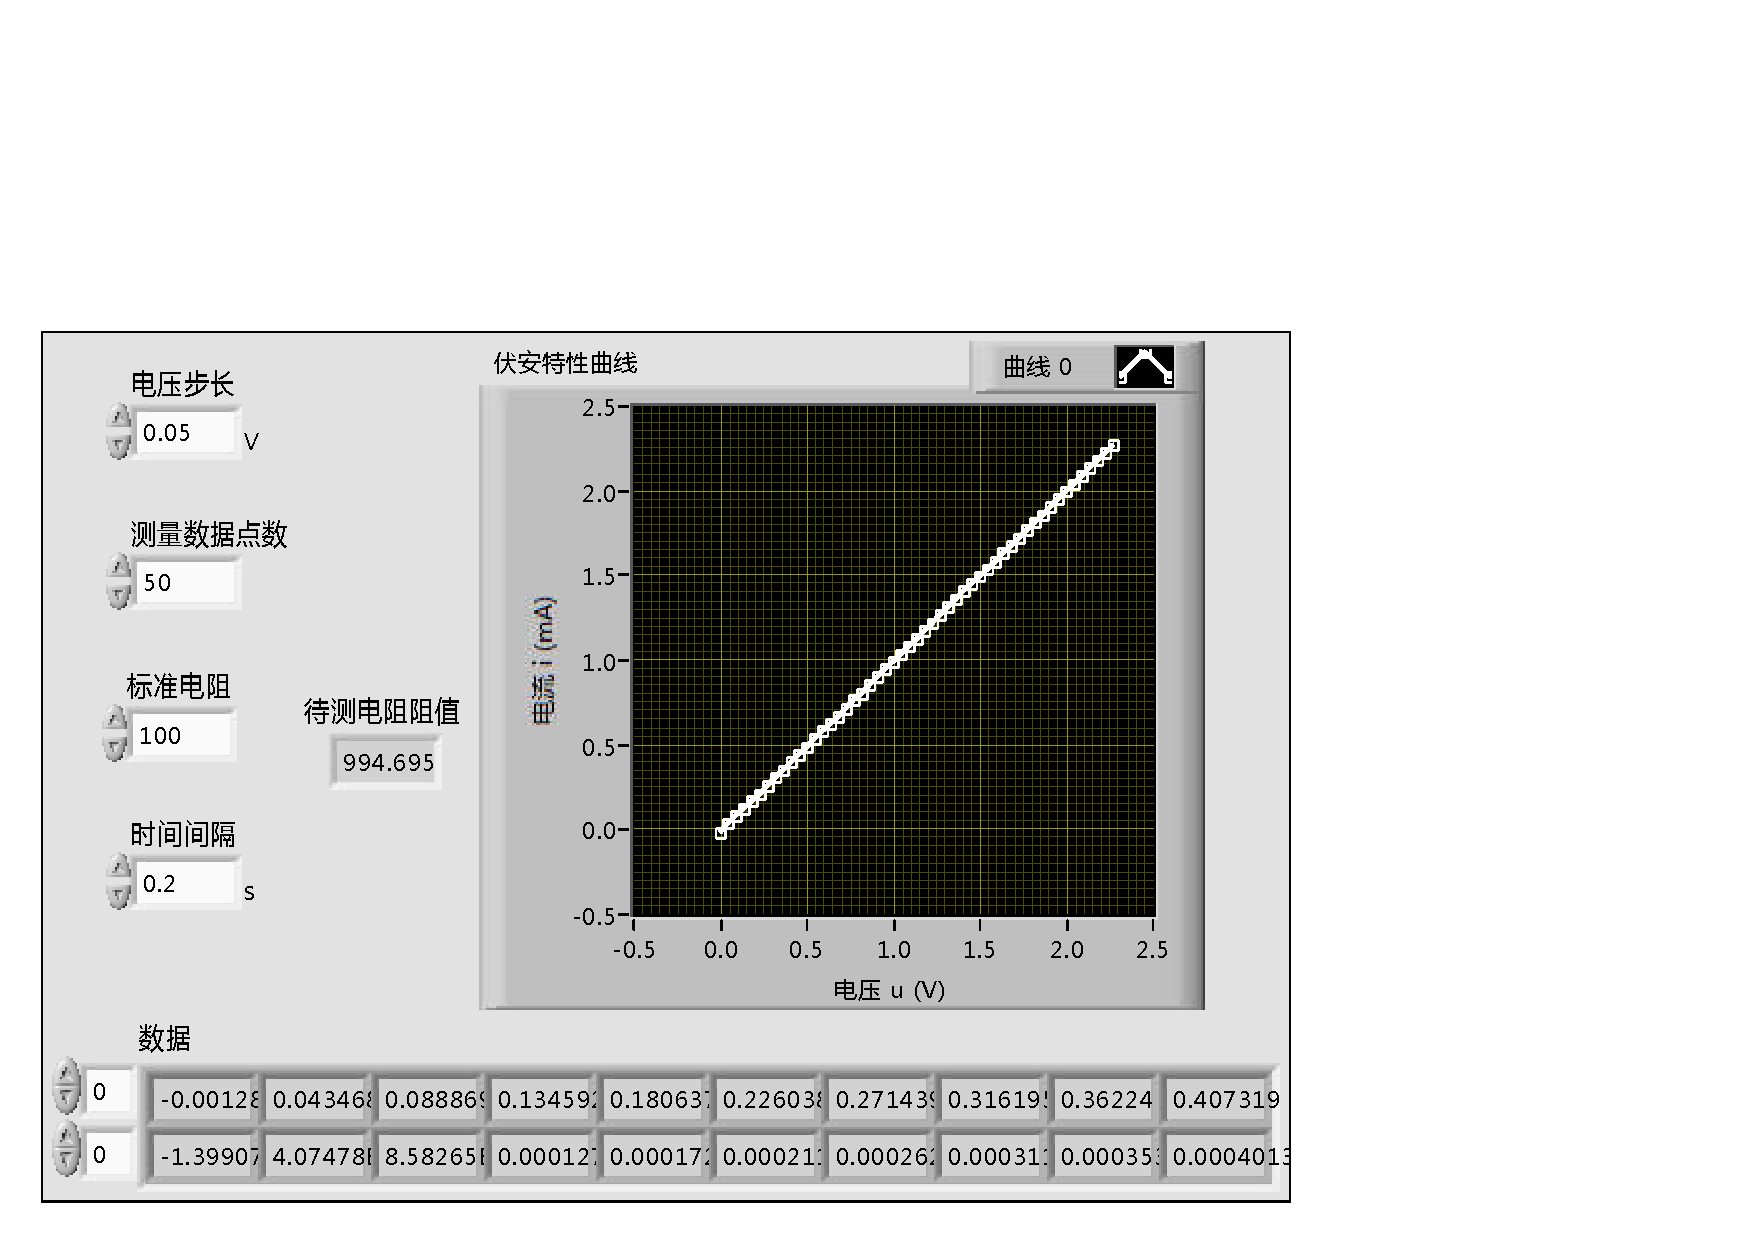
\includegraphics[height=150pt]{assets/测量伏安曲线__1K欧电阻.pdf}
        \caption{前面板}
    \end{subfigure}\hfill
    \begin{subfigure}[b]{0.55\columnwidth}\centering
        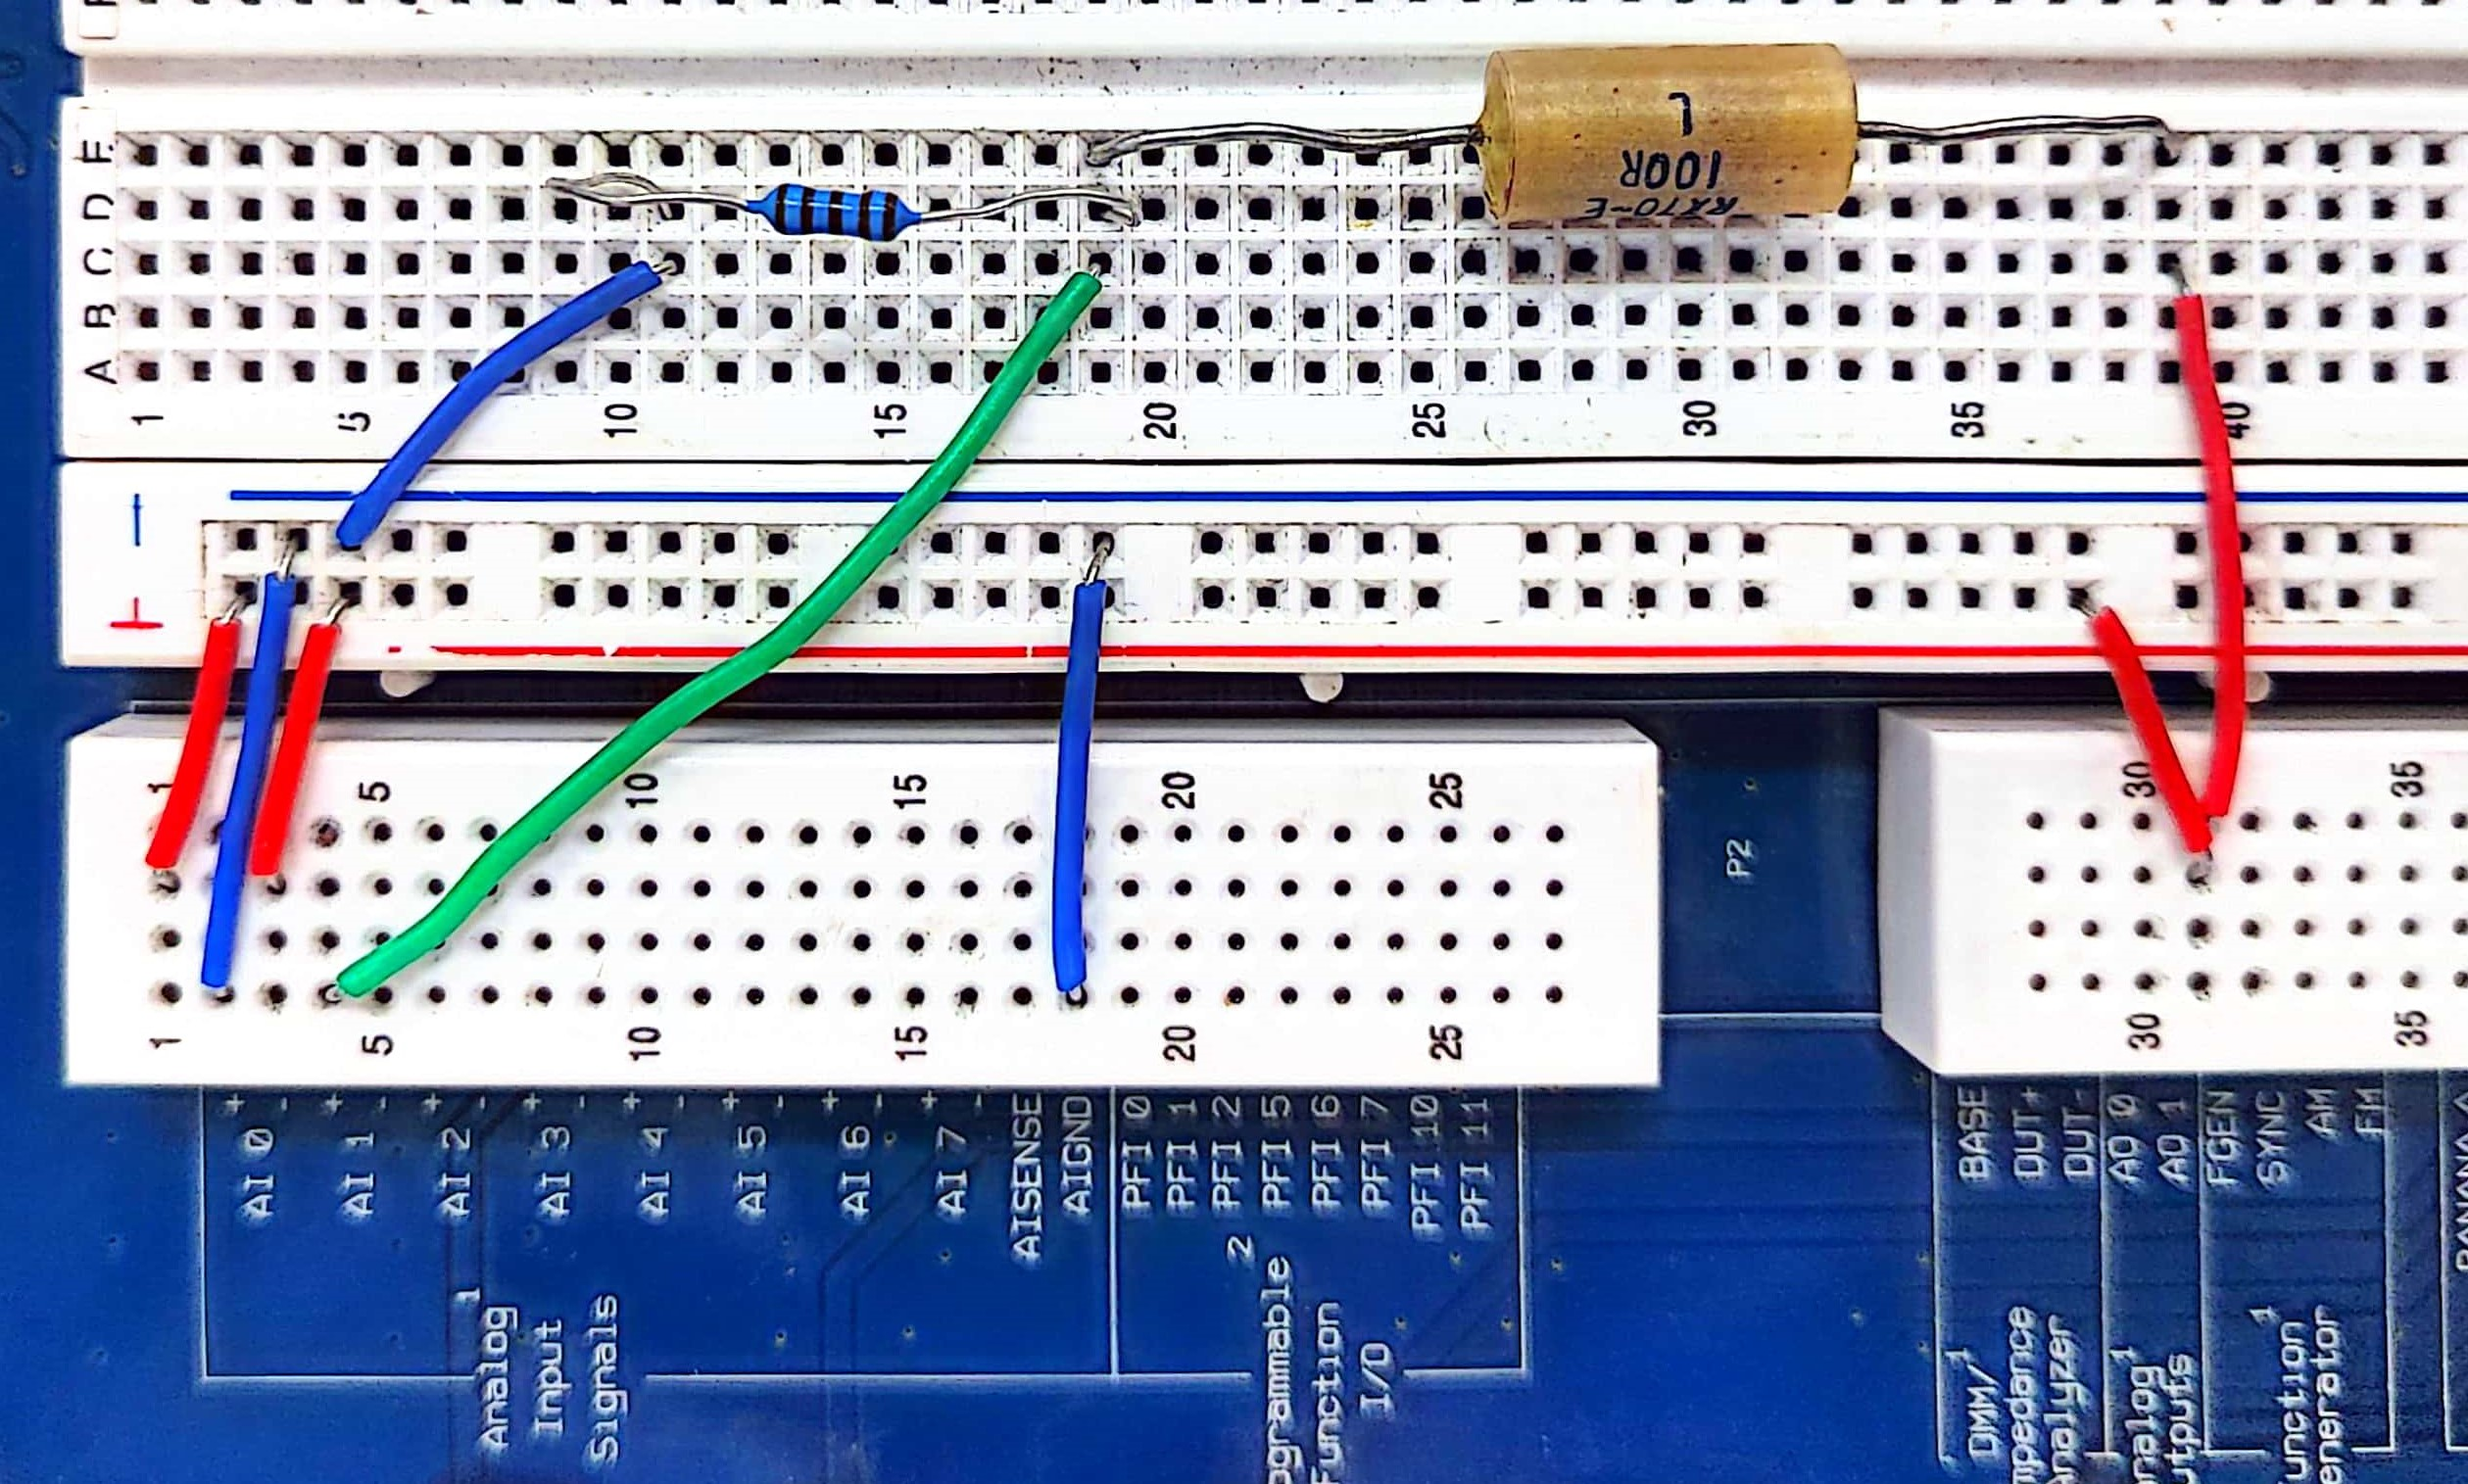
\includegraphics[height=150pt]{assets/测量伏安曲线__1K欧电阻.jpg}
        \caption{实际电路连接}
    \end{subfigure}
    \caption{测量 $1 \kO$ 电阻的伏安曲线}
    \label{测量1K欧电阻的伏安曲线}
\end{figure}

\begin{table}[H]\centering
%\renewcommand{\arraystretch}{1.5} % 调整行间距为 1.5 倍
%\setlength{\tabcolsep}{1.5mm} % 调整列间距
\caption{$1 \KO$ 电阻的伏安数据}
\label{1K欧电阻伏安数据}
\begin{tabular}{|ll|ll|ll|}
    \hline
    电压 (V)  & 电流 (A)   & 电压 (V)  & 电流 (A)   &电压 (V)  & 电流 (A) \\ \hline
    -0.00128796 & -0.00001399   & 0.770204 & 0.000768448 & 1.54234 & 0.00153801  \\
    0.0434688   & 0.000040748    & 0.816571 & 0.000803867 & 1.58806 & 0.00158309  \\
    0.0888696   & 0.000085827    & 0.860684 & 0.000855386 & 1.63218 & 0.0016346   \\
    0.134592    & 0.000127685 & 0.906084 & 0.000903684 & 1.67887 & 0.00167646  \\
    0.180637    & 0.000172764 & 0.951163 & 0.000951983 & 1.72395 & 0.00172154  \\
    0.226038    & 0.000211403 & 0.99753  & 0.000993842 & 1.76903 & 0.00176984  \\
    0.271439    & 0.000262922 & 1.04293  & 0.0010357   & 1.81475 & 0.00181492  \\
    0.316195    & 0.00031122  & 1.08801  & 0.001084    & 1.86047 & 0.00185678  \\
    0.36224     & 0.000353079 & 1.1347   & 0.00112586  & 1.90458 & 0.00190508  \\
    0.407319    & 0.000401378 & 1.17913  & 0.00117416  & 1.95095 & 0.00195338  \\
    0.453364    & 0.000446457 & 1.22453  & 0.00121924  & 1.99603 & 0.00199845  \\
    0.498443    & 0.000488316 & 1.26929  & 0.00127075  & 2.04143 & 0.00204031  \\
    0.5432      & 0.000539834 & 1.31469  & 0.00131583  & 2.08651 & 0.00208861  \\
    0.5886      & 0.000584913 & 1.36042  & 0.00136091  & 2.13191 & 0.00213691  \\
    0.634967    & 0.000626772 & 1.40517  & 0.00141243  & 2.17731 & 0.00218199  \\
    0.680368    & 0.000668631 & 1.45057  & 0.00145107  & 2.22336 & 0.00222385  \\
    0.725447    & 0.000716929 & 1.4963   & 0.00149615  & 2.26876 & 0.00227215 \\
    \hline
\end{tabular}
\end{table}

由 LabVIEW 程序中的线性拟合(前面板上的结果),可得电阻的测量值为 $R = 994.695\ \Omega$。我们在 Matlab 中用最小二乘法对函数 $i = \frac{1}{R}u$ 进行拟合,得到 $R = 1000.7715 \ \Omega$,两者结果基本吻合。

%\begin{figure}[H]\centering
%\begin{subfigure}[b]{0.5\columnwidth}\centering
%    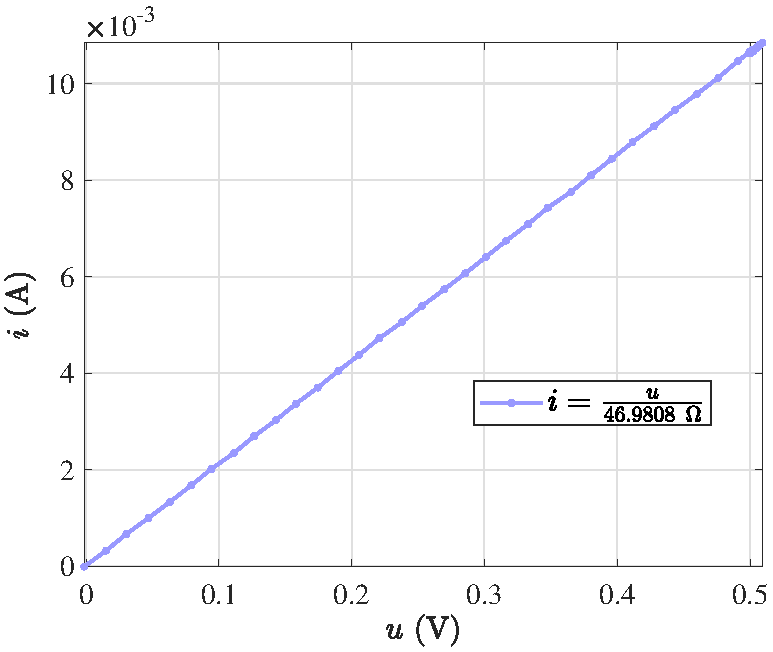
\includegraphics[height=200pt]{assets/51欧电阻.pdf}
%    \caption{$51 \ \Omega$ 电阻}
%\end{subfigure}\hfill
%\begin{subfigure}[b]{0.5\columnwidth}\centering
%    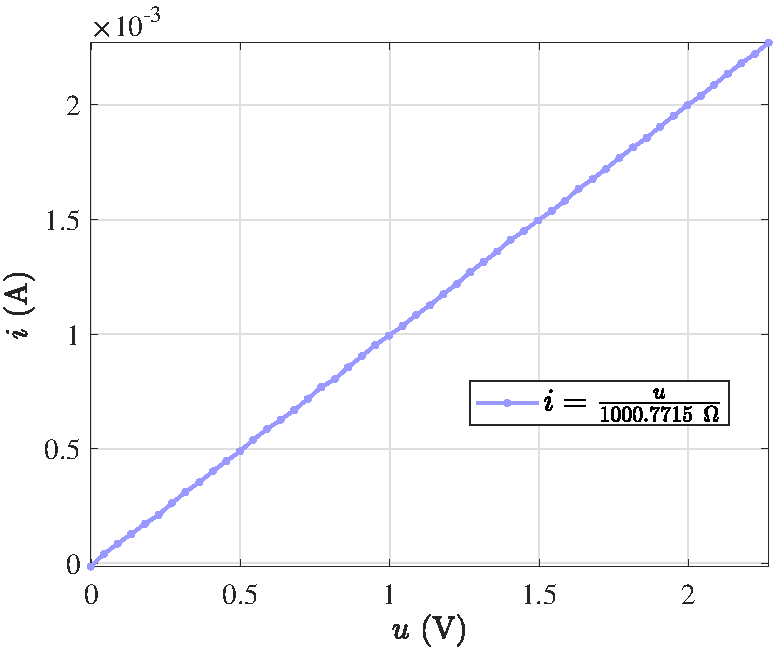
\includegraphics[height=200pt]{assets/1K欧电阻.pdf}
%    \caption{$1 \kO$ 电阻}
%\end{subfigure}
%\caption{Matlab 最小二乘拟合结果}
%\label{Matlab 最小二乘拟合结果}
%\end{figure}

\newpage
\subsection{整流二极管}

待测元件是导通电压约为 0.6 V 的整流二极管,前面板参数设置和电路连接方式见图 \ref{测量整流二极管的伏安曲线},所得 $u$-$i$ 数据如表 \ref{整流二极管伏安数据} 所示。

\begin{figure}[H]\centering
    \begin{subfigure}[b]{0.45\columnwidth}\centering
        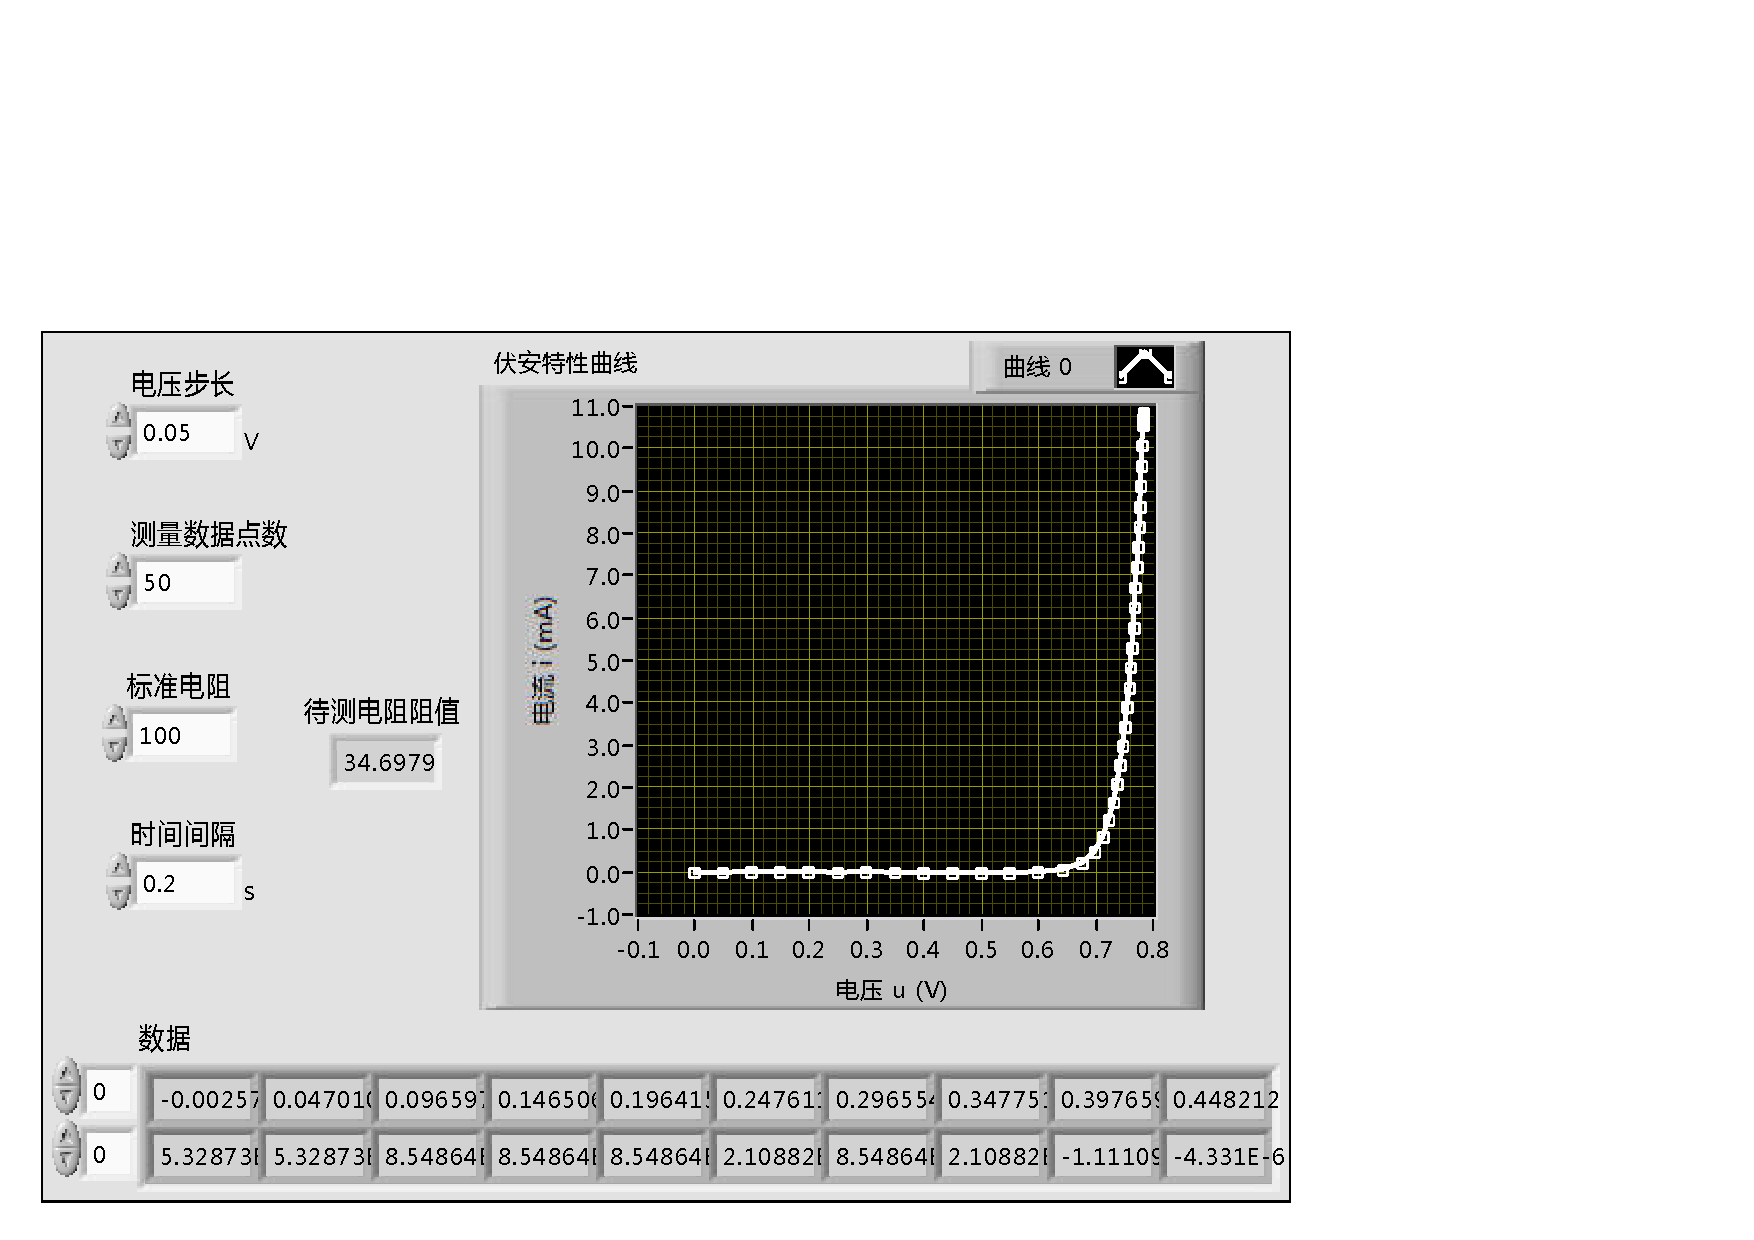
\includegraphics[height=150pt]{assets/测量伏安曲线__整流二极管.pdf}
        \caption{前面板}
    \end{subfigure}\hfill
    \begin{subfigure}[b]{0.55\columnwidth}\centering
        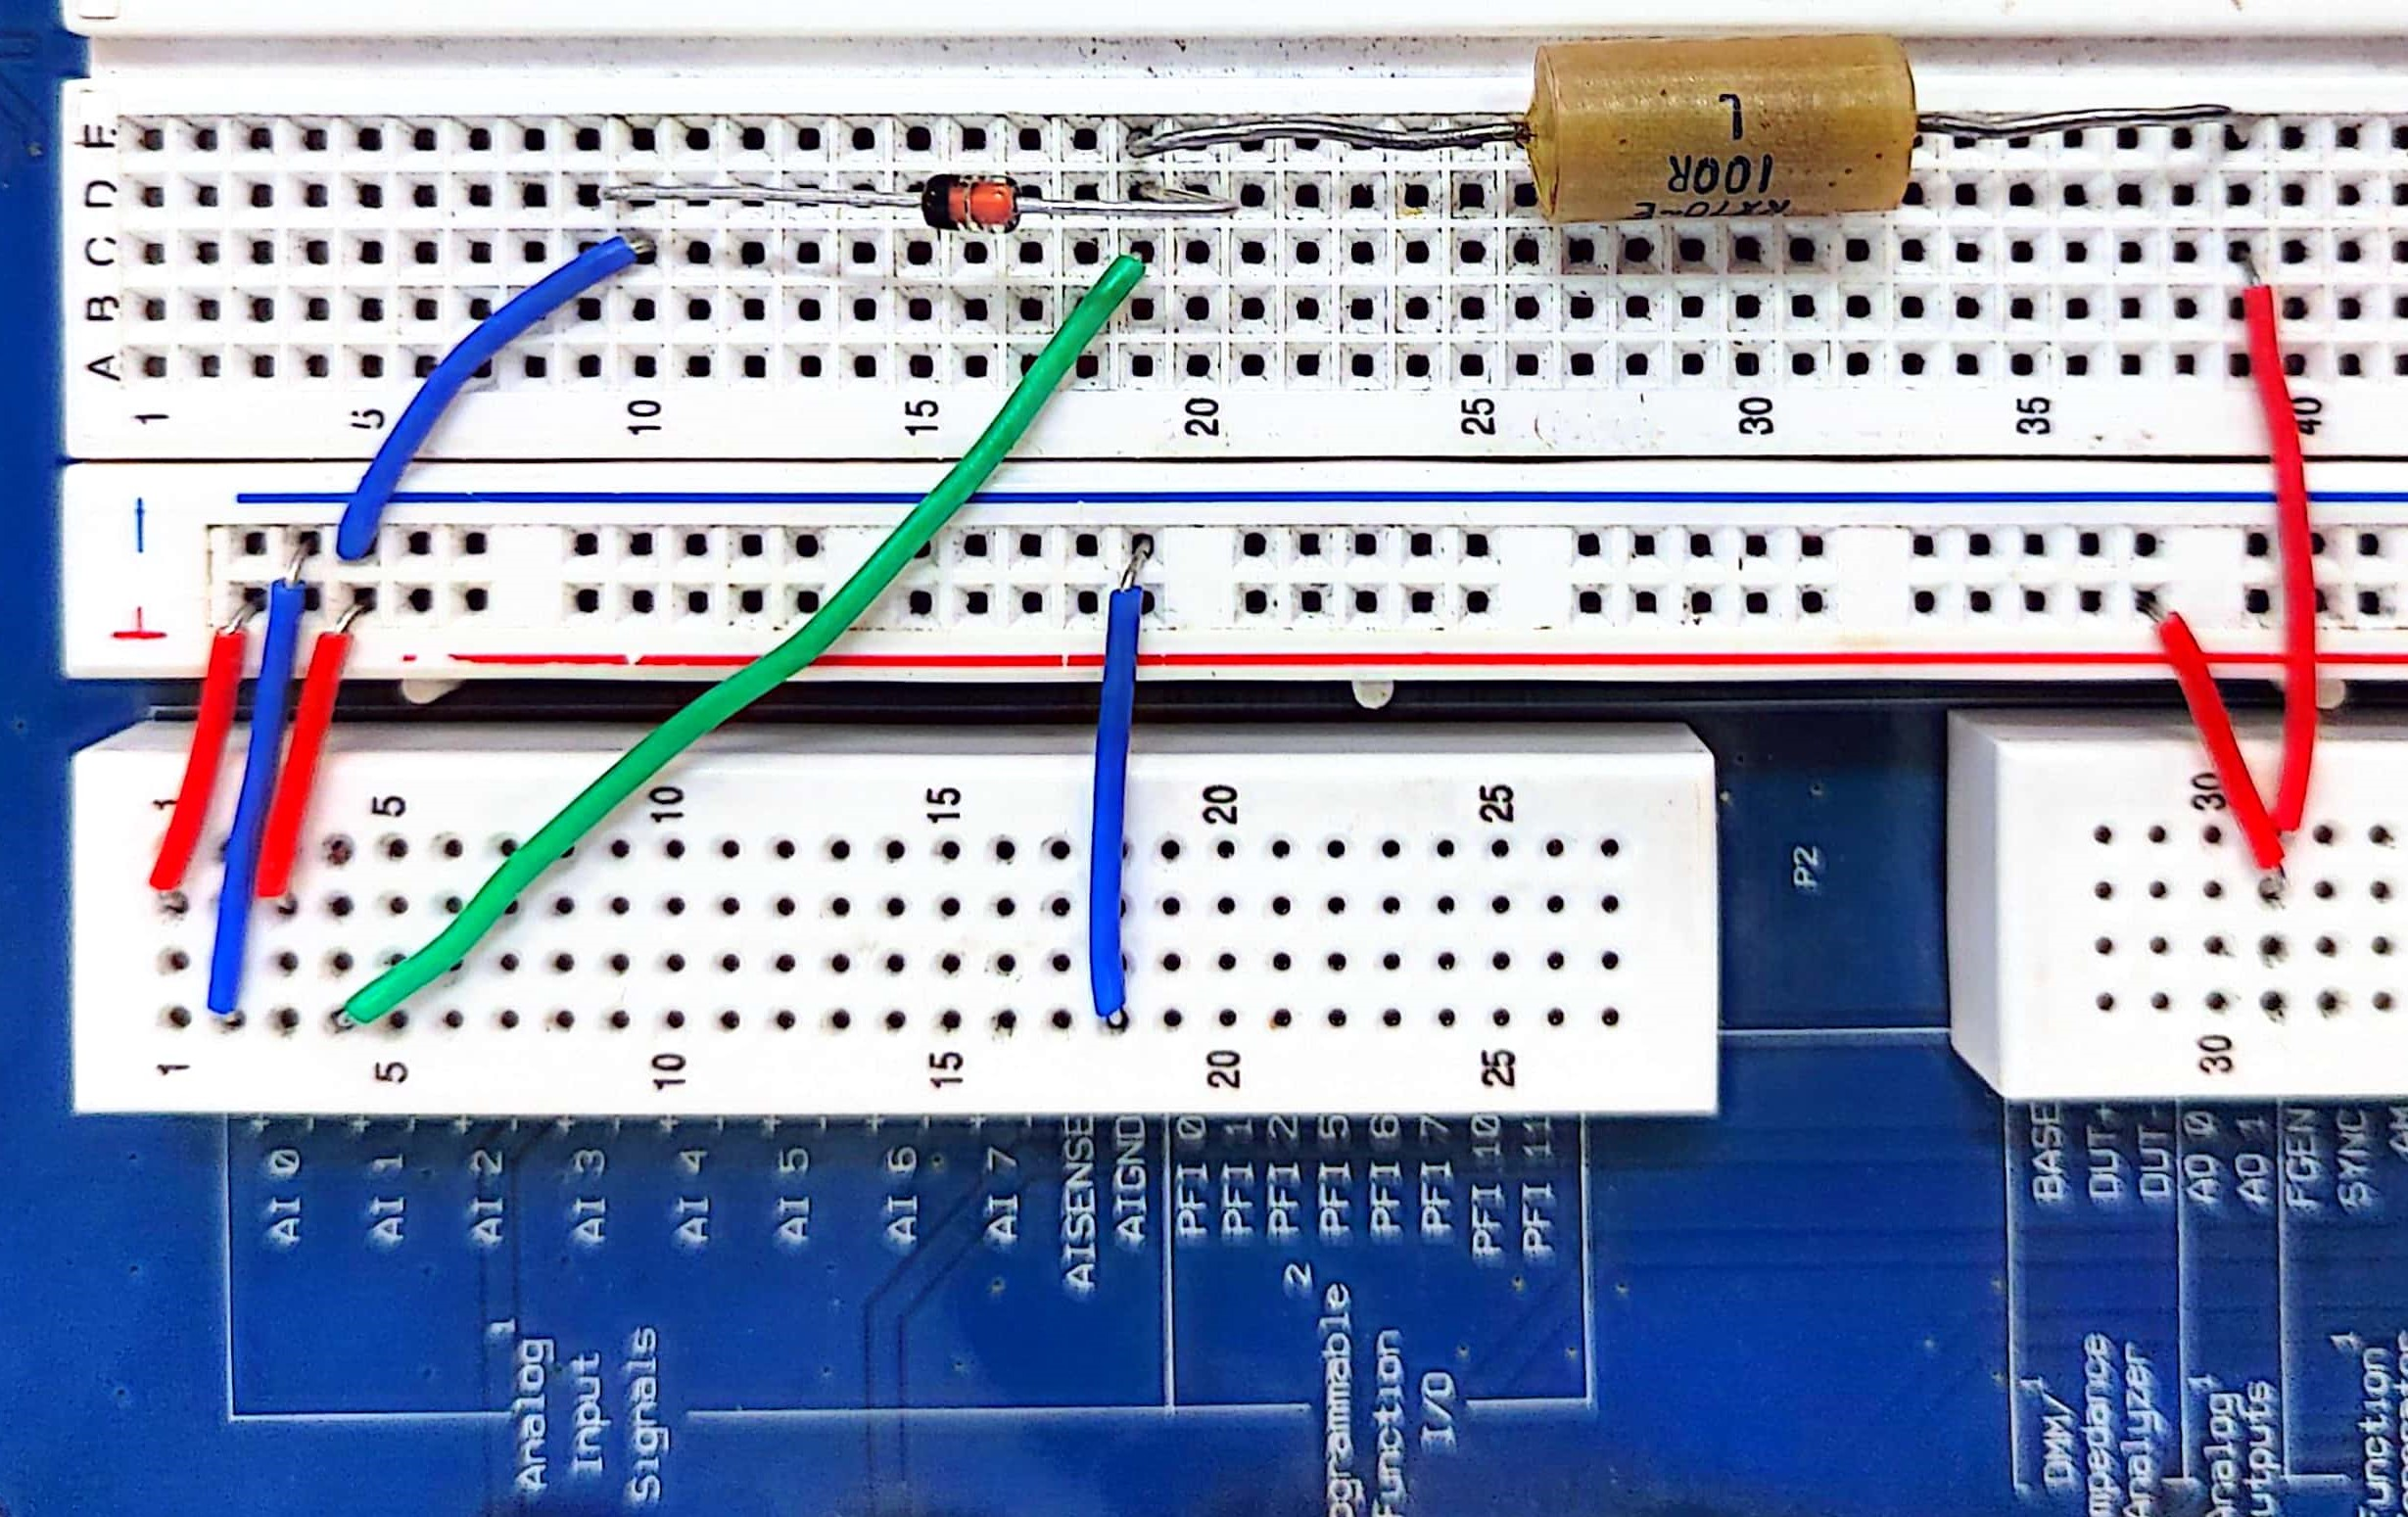
\includegraphics[height=150pt]{assets/测量伏安曲线__整流二极管.jpg}
        \caption{实际电路连接}
    \end{subfigure}
    \caption{测量整流二极管的伏安曲线}
    \label{测量整流二极管的伏安曲线}
\end{figure}

\begin{table}[H]\centering
%\renewcommand{\arraystretch}{1.5} % 调整行间距为 1.5 倍
%\setlength{\tabcolsep}{1.5mm} % 调整列间距
\caption{整流二极管的伏安数据}
\label{整流二极管伏安数据}
\begin{tabular}{|ll|ll|ll|}
    \hline
    电压 (V)  & 电流 (A)   & 电压 (V)  & 电流 (A)   &电压 (V)  & 电流 (A) \\ \hline
    -0.00257593 & 5.33E-06    & 0.721583 & 0.00124499 & 0.777612 & 0.00912091  \\
    0.0470107   & 5.33E-06    & 0.730599 & 0.00165714 & 0.779544 & 0.00959424  \\
    0.0965974   & 8.55E-06    & 0.736395 & 0.00208861 & 0.78051  & 0.0100772   \\
    0.146506    & 8.55E-06    & 0.741869 & 0.00253296 & 0.781476 & 0.0105602   \\
    0.196415    & 8.55E-06    & 0.746055 & 0.00298697 & 0.783086 & 0.0108597   \\
    0.247611    & 2.11E-06    & 0.750563 & 0.00344098 & 0.782442 & 0.0107888   \\
    0.296554    & 8.55E-06    & 0.754105 & 0.0038982  & 0.782764 & 0.0107405   \\
    0.347751    & 2.11E-06    & 0.757969 & 0.00435865 & 0.78212  & 0.0107083   \\
    0.397659    & -1.11E-06   & 0.759901 & 0.0048352  & 0.783086 & 0.0106794   \\
    0.448212    & -4.33E-06   & 0.762477 & 0.00530531 & 0.78212  & 0.0106697   \\
    0.498765    & -7.55E-06   & 0.765697 & 0.00577219 & 0.78212  & 0.0106536   \\
    0.547707    & -1.11E-06   & 0.766663 & 0.00625196 & 0.782442 & 0.0106375   \\
    0.596972    & 8.55E-06    & 0.768273 & 0.00672529 & 0.781476 & 0.0106311   \\
    0.640763    & 6.65E-05    & 0.771493 & 0.00720184 & 0.78212  & 0.0106214   \\
    0.675216    & 0.000221063 & 0.773425 & 0.00767517 & 0.78212  & 0.0106182   \\
    0.697434    & 0.000494755 & 0.775357 & 0.00815493 & 0.782442 & 0.0106085   \\
    0.711923    & 0.000848946 & 0.776968 & 0.0086347  & 0.782442 & 0.0106021  \\
    \hline
\end{tabular}
\end{table}

整流二极管并不是线性元件,容易看出其伏安特性曲线并非直线,而且在正向电压大于导通电压时,电流才会显著增大。我们在 Matlab 中作出其伏安曲线,如图 \ref{二极管} (a)。


\subsection{发光二极管}


待测元件是压降约为 1.5 V 的发光二极管,前面板参数设置和电路连接方式见图 \ref{测量发光二极管的伏安曲线},所得 $u$-$i$ 数据如表 \ref{发光二极管伏安数据} 所示。得到数据后,类似地,我们也在 Matlab 中作出发光二极管的伏安曲线,如图 \ref{二极管} (b)。

\begin{figure}[H]\centering
    \begin{subfigure}[b]{0.45\columnwidth}\centering
        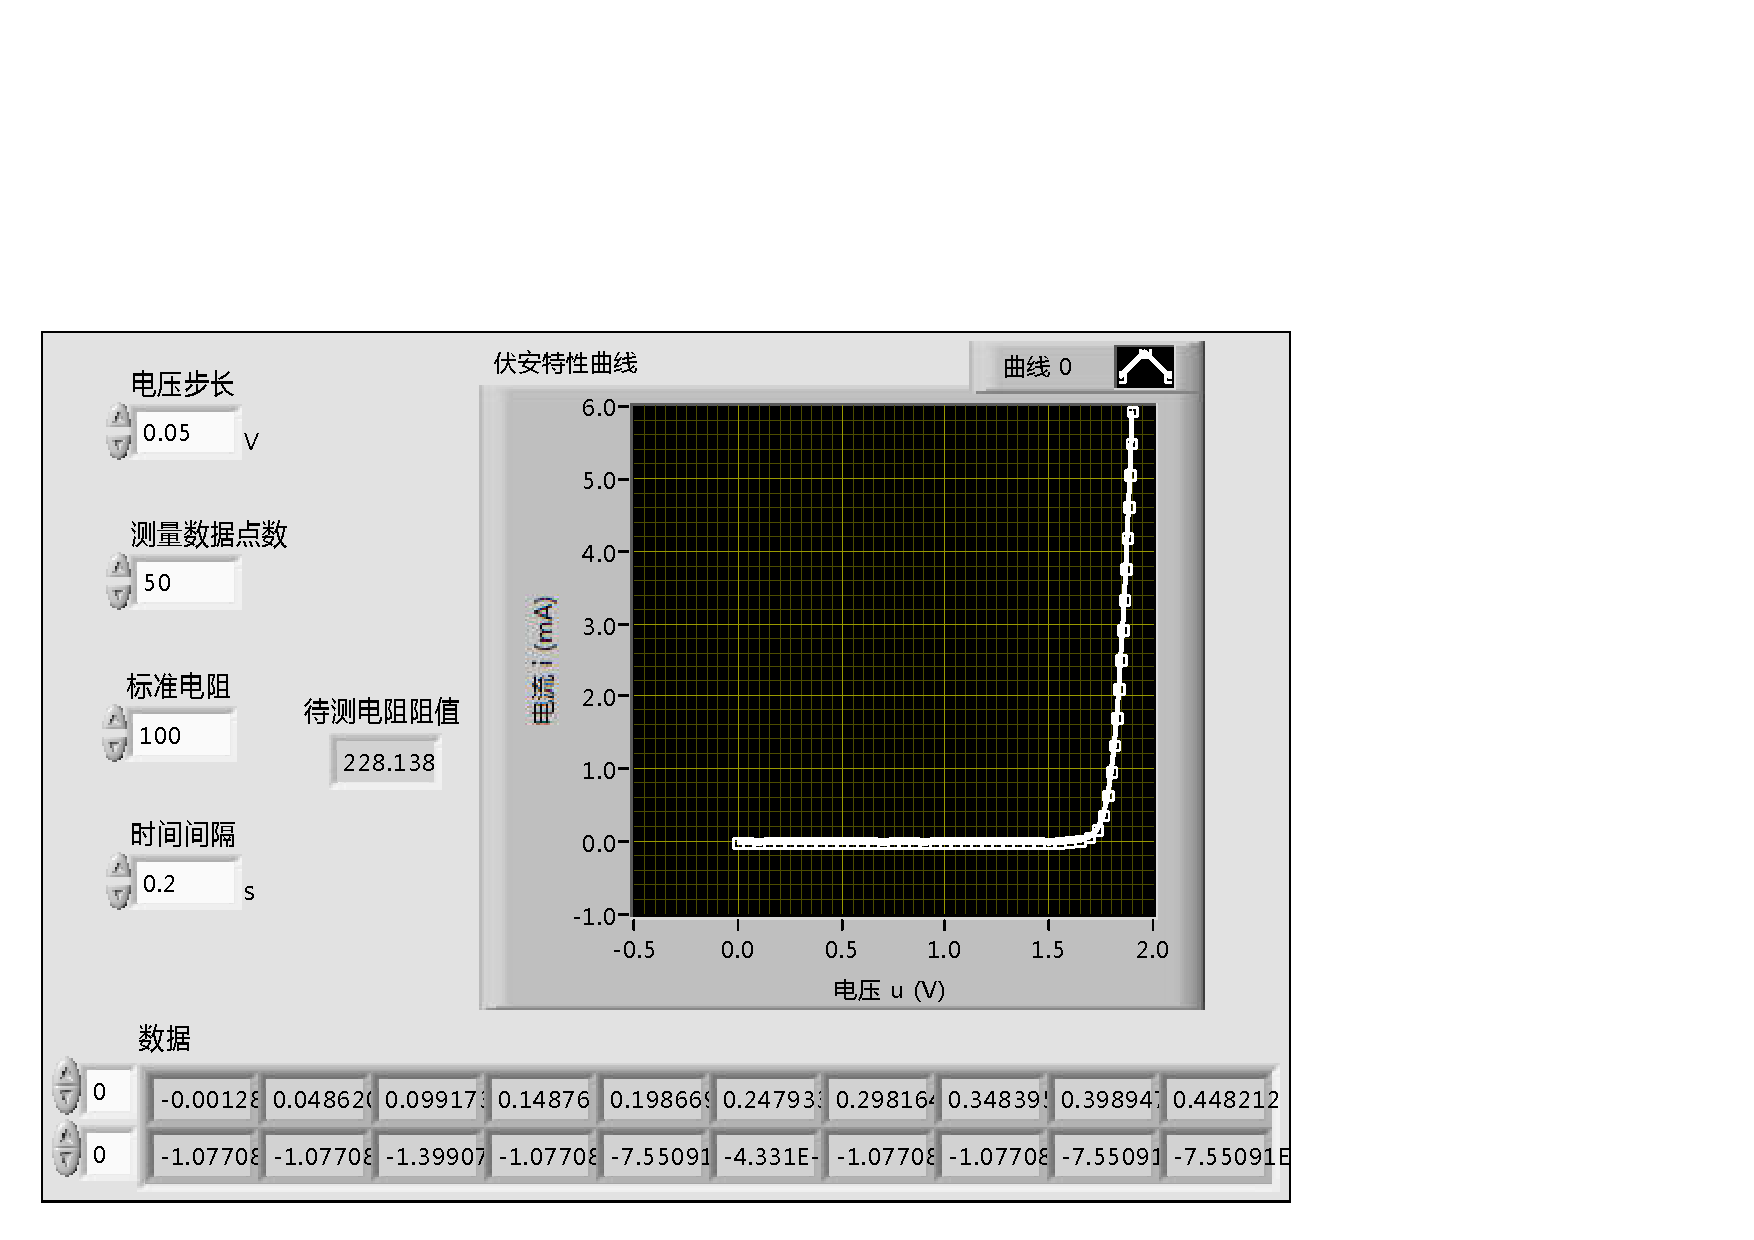
\includegraphics[height=130pt]{assets/测量伏安曲线__发光二极管.pdf}
        \caption{前面板}
    \end{subfigure}\hfill
    \begin{subfigure}[b]{0.55\columnwidth}\centering
        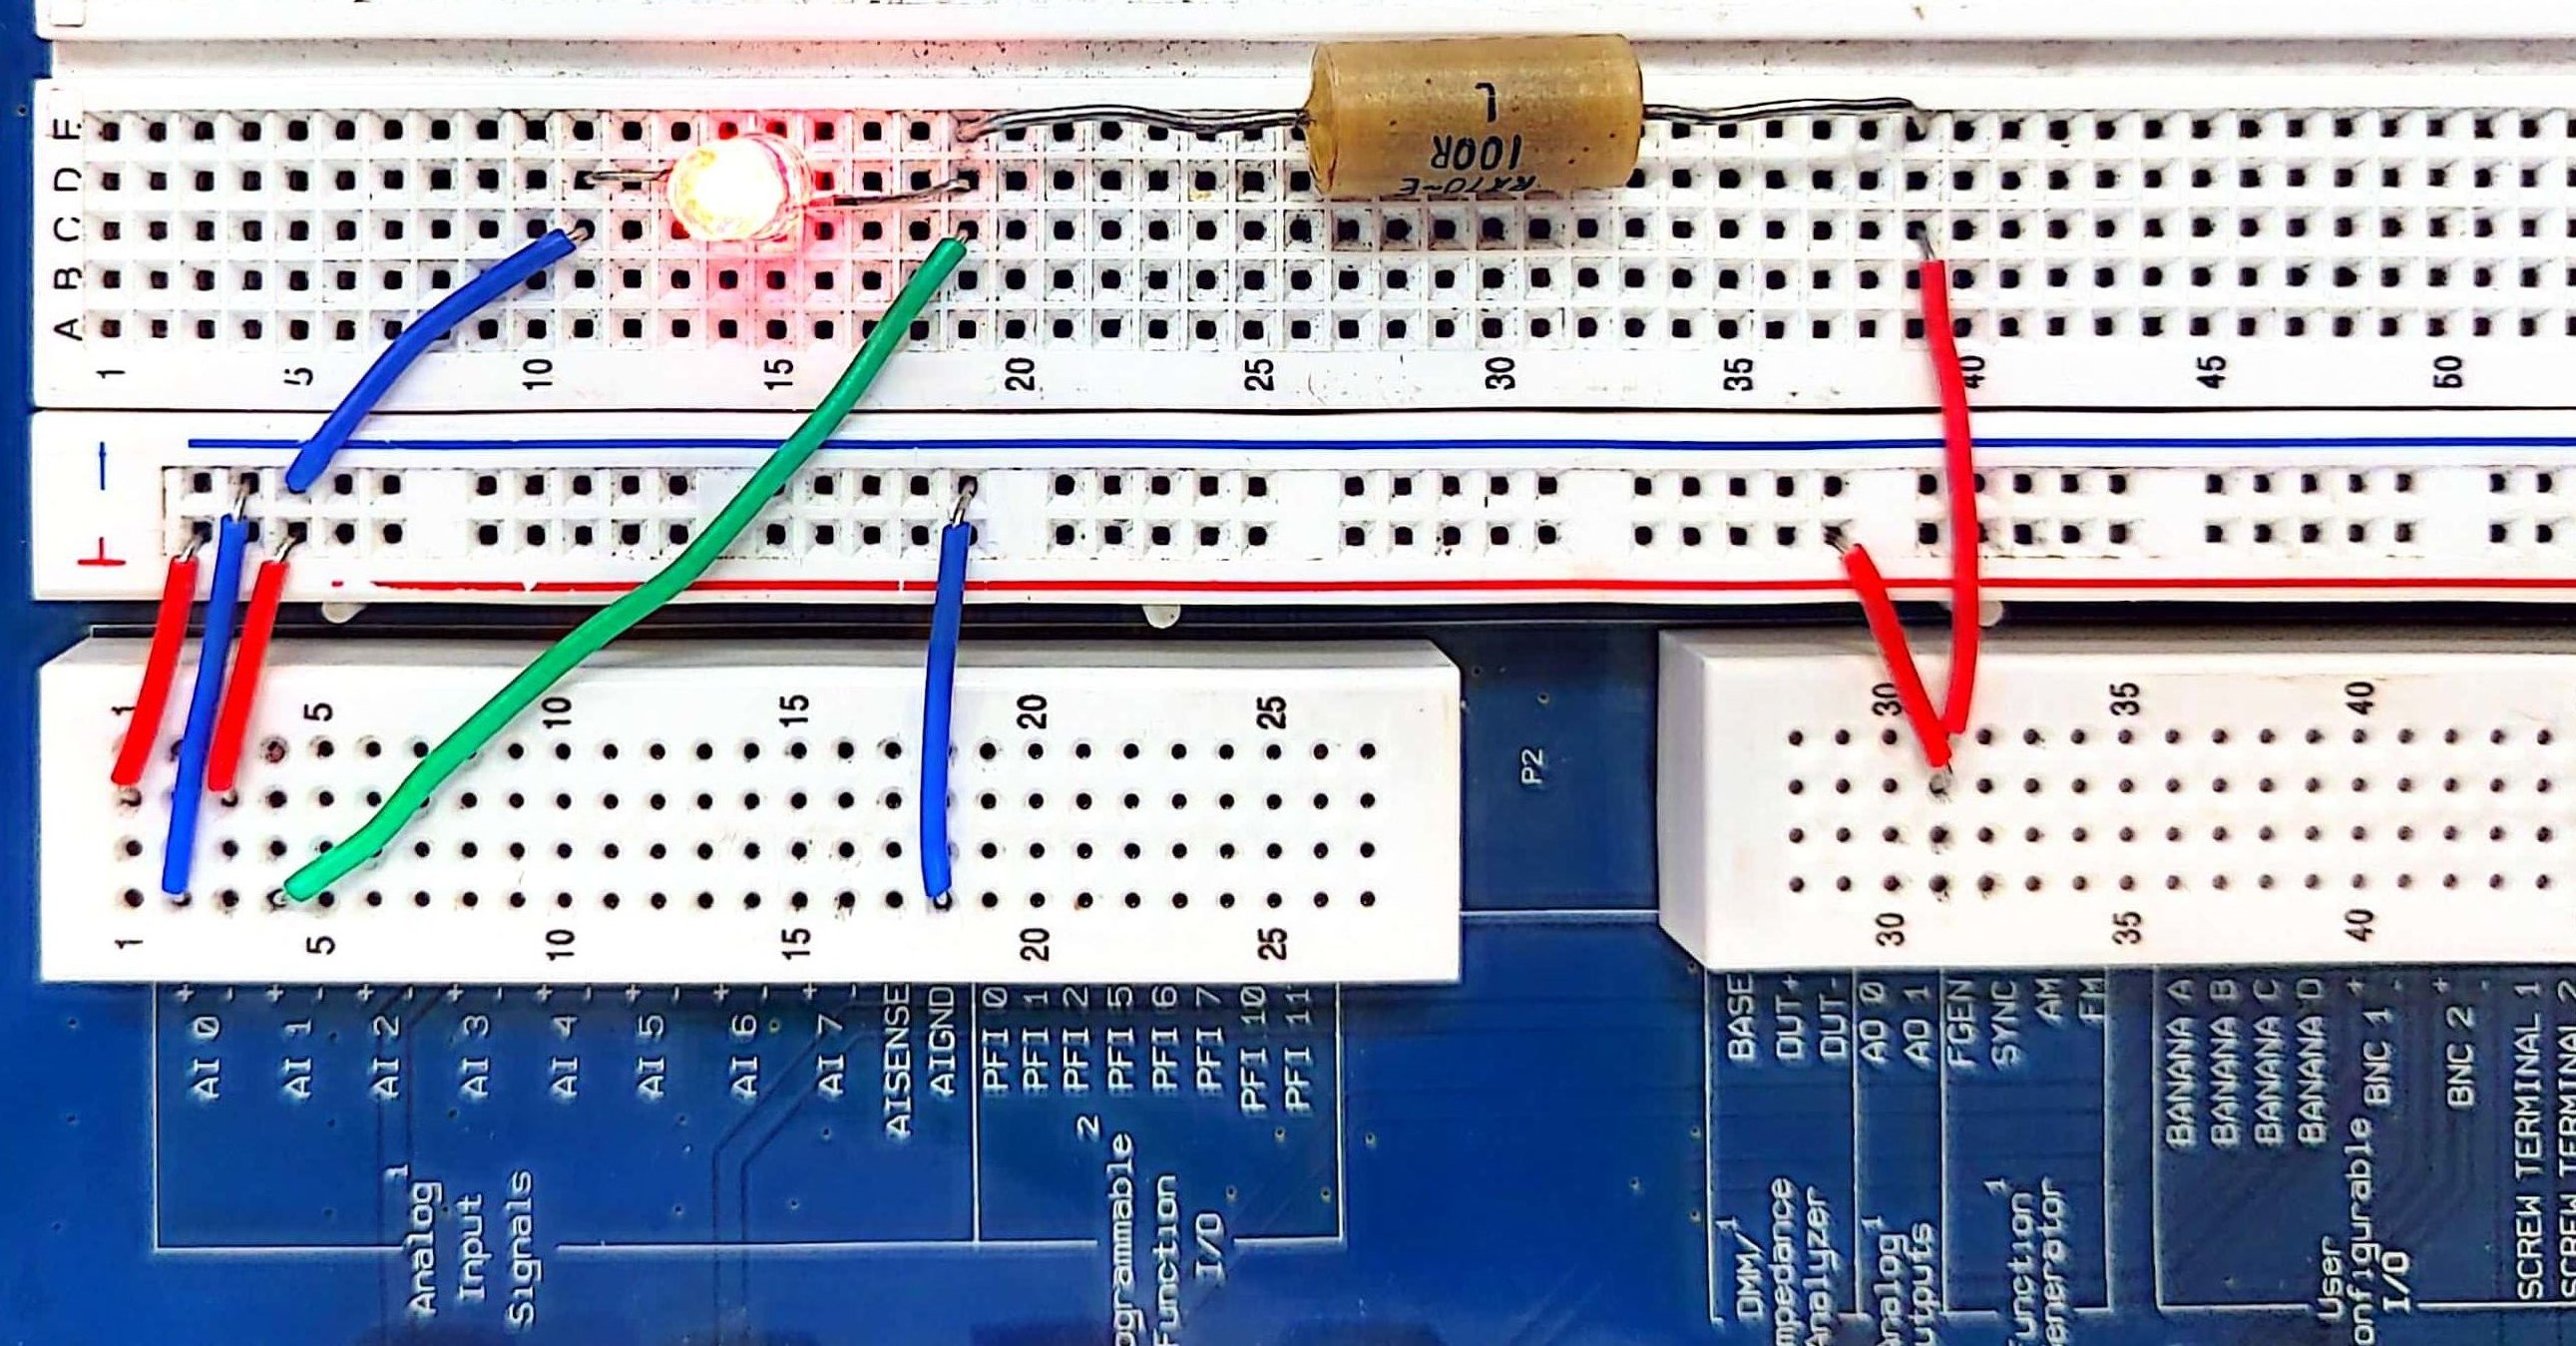
\includegraphics[height=130pt]{assets/测量伏安曲线__发光二极管.jpg}
        \caption{实际电路连接}
    \end{subfigure}
    \caption{测量发光二极管的伏安曲线}
    \label{测量发光二极管的伏安曲线}
\end{figure}
\vspace*{-5mm}
\begin{table}[H]\centering
%\renewcommand{\arraystretch}{1.5} % 调整行间距为 1.5 倍
%\setlength{\tabcolsep}{1.5mm} % 调整列间距
\caption{发光二极管的伏安数据}
\label{发光二极管伏安数据}
\begin{tabular}{|ll|ll|ll|}
    \hline
    电压 (V)  & 电流 (A)   & 电压 (V)  & 电流 (A)   &电压 (V)  & 电流 (A) \\ \hline
    -0.00128796 & -1.08E-05 & 0.848448 & -7.55E-06 & 1.6911  & 6.65E-05     \\
    0.0486207   & -1.08E-05 & 0.899    & -1.40E-05 & 1.73038 & 0.000169544  \\
    0.0991733   & -1.40E-05 & 0.948265 & -1.08E-05 & 1.76001 & 0.000369179  \\
    0.14876     & -1.08E-05 & 0.998174 & -7.55E-06 & 1.7819  & 0.000646091  \\
    0.198669    & -7.55E-06 & 1.04873  & -1.08E-05 & 1.79897 & 0.000974522  \\
    0.247933    & -4.33E-06 & 1.09799  & -1.08E-05 & 1.81282 & 0.00133515   \\
    0.298164    & -1.08E-05 & 1.14854  & -7.55E-06 & 1.82505 & 0.00171188   \\
    0.348395    & -1.08E-05 & 1.19781  & -7.55E-06 & 1.83503 & 0.00210471   \\
    0.398947    & -7.55E-06 & 1.24868  & -7.55E-06 & 1.84373 & 0.00251364   \\
    0.448212    & -7.55E-06 & 1.29827  & -7.55E-06 & 1.85274 & 0.00291935   \\
    0.498443    & -7.55E-06 & 1.34786  & -7.55E-06 & 1.86144 & 0.00333472   \\
    0.548351    & -7.55E-06 & 1.39809  & -7.55E-06 & 1.8682  & 0.00376297   \\
    0.59826     & -7.55E-06 & 1.448    & -7.55E-06 & 1.87432 & 0.004188     \\
    0.648491    & -7.55E-06 & 1.49919  & -1.40E-05 & 1.88172 & 0.00461946   \\
    0.699365    & -1.40E-05 & 1.54781  & -7.55E-06 & 1.88752 & 0.00505415   \\
    0.74863     & -1.08E-05 & 1.59676  & 5.33E-06  & 1.89364 & 0.00548884   \\
    0.797895    & -1.08E-05 & 1.64538  & 1.82E-05  & 1.89911 & 0.00592997  \\
    \hline
\end{tabular}
\end{table}

\begin{figure}[H]\centering
\begin{subfigure}[b]{0.5\columnwidth}\centering
    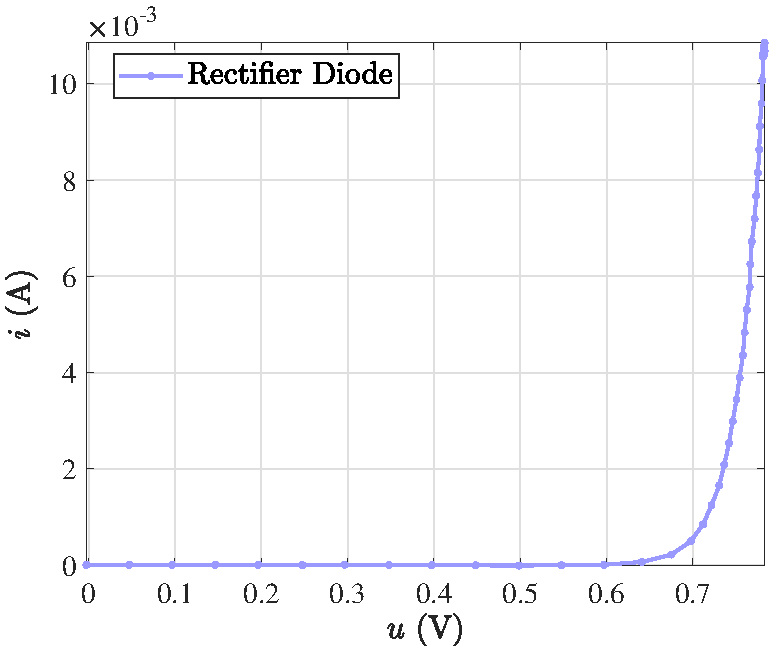
\includegraphics[height=170pt]{assets/整流二极管.pdf}
    \caption{ 整流二极管 (Rectifier Diode) }
\end{subfigure}\hfill
\begin{subfigure}[b]{0.5\columnwidth}\centering
    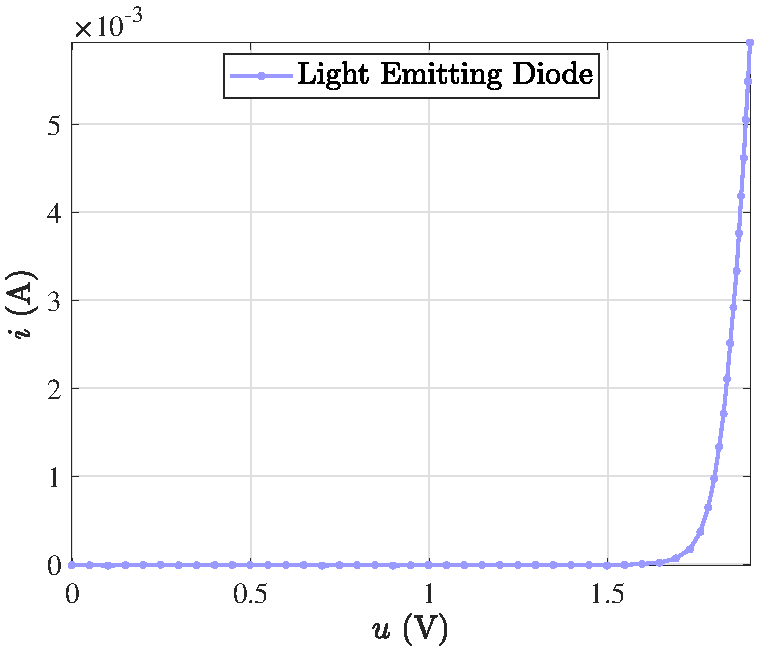
\includegraphics[height=170pt]{assets/发光二极管.pdf}
    \caption{ 发光二极管 (Light Emitting Diode) }
\end{subfigure}
\caption{二极管的伏安特性曲线}
\label{二极管}
\end{figure}

\section{思考题}

\subsection{虚拟仪器系统与传统仪器有什么区别?请简要说明}

虚拟仪器基于计算机系统,通过编程手段,将计算机的控制能力用于实际仪器,实现了对实验仪器的高级操控,便于自动化控制。这突破了传统实验的读数不便、实验操作自动化程度低、实验成本高昂、仪器功能局限性高等限制,极大节省了开展实验的时间和经济成本,大大提高了实验效率。

一个非常典型的例子便是本次实验的“测量伏安曲线”一节。在实验中,我们只需设置参数“电压步长”和“数据点”的值,便能通过虚拟仪器的自动化控制,迅速而准确地得到成百上千个实验数据点。如果换作传统实验,在每次获取新数据点时都需要重新调整实验仪器、关注量表的量程,这将消耗极大的精力和时间。

虚拟仪器系统还可以通过软件的更新和升级不断扩展和增强功能,而传统仪器
则需要更换新的设备。但虚拟仪器也有缺点:比如需要使用者有一定的编程功底,有时这对实验者的要求很高;又如虚拟仪器需要实际仪器的辅助,受到实际仪器的限制。



\subsection{本实验内容 3 中的电压输出和采集哪个先执行?}

物理通道的相关程序在运行前就已经搭建完成,因此,从代码的角度来讲,在开始运行时,电压输出和采集两个程序是并行的,具体的先后顺序取决于底层编译器的编译结果。但从实际应用的层面考虑,可以采用电压输出先执行、电压采集后执行的策略,待电路参数(电压输出值)发生变化并达到稳定时,再对电压进行采集,使测量结果更精确。

\section{实验总结与思考}

在本次实验中,我学习了如何使用 LabVIEW 开发平台,运行了一些简单的例子,并将 LabVIEW 与实际电路相结合,实现了对伏安特性曲线测量的自动化控制,包括 $51 \ \Omega$ 电阻、$1 \KO$ 电阻、整流二极管和发光二极管。
得益于郭思明老师的耐心指导和实验讲义的详尽,即便此前从未听闻过 LabVIEW 和 NI ELVIS II$^+$,我也能较为高效地完成全部实验内容。这种将模拟、仿真与实际电路与元件相结合的开发模式,极大地提高了实验和开发效率,为我们电子系学生今后的实验和研究工作提供了独特的思路。

LabVIEW 的图形化编程让我想起了单片机中类似的图形化开发软件,例如 Arduino 语言下的 Mixly、Mind+ 等软件。它们都通过将编程代码图形化,降低了对开发者编程水平的要求,在某些方面使得开发更为高效

此次实验,我利用了 Matlab 软件对实验数据作进一步的处理和分析,这为数据处理和可视化带来了极大方便。在今后的实验和研究工作中,我还会继续深入学习和应用这些计算软件,增强自己的科学计算能力。

在数据处理的过程中,我还发现标定值为 $51 \ \Omega$ 的电阻,所测得的阻值偏小。这可能与测压电路的并联分流有关,值得进一步探究并寻求改进方法。




% --------------------------- 附录 --------------------------- %
% >> ------------------------ 附录 ------------------------ << %


\newpage
\appendix
% section 标题自定义设置 
\titleformat{\section}[hang]{\normalfont\huge\bfseries\centering}{}{20pt}{}
\titlespacing*{\section}{0pt}{-25pt}{8pt} % 控制上方空白的大小

% 附录 A
\section*{附录 A\hspace*{20pt} 原始数据记录与部分实验照片}
\addcontentsline{toc}{section}{附录 A\hspace*{6pt} 原始数据记录与部分实验照片}    
\thispagestyle{fancy} 


\begin{figure}[H]\centering
    \begin{subfigure}[b]{0.72\columnwidth}\centering
        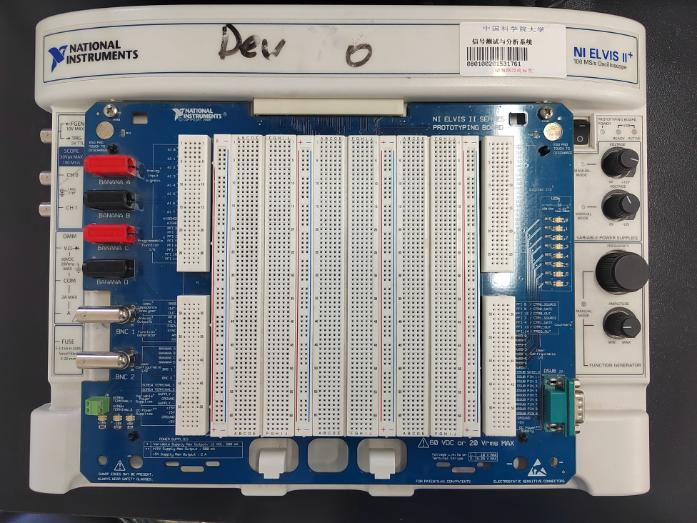
\includegraphics[height=250pt]{assets/附录/IMG_20241015_130009.jpg}
    \end{subfigure}\hfill
    \begin{subfigure}[b]{0.28\columnwidth}\centering
        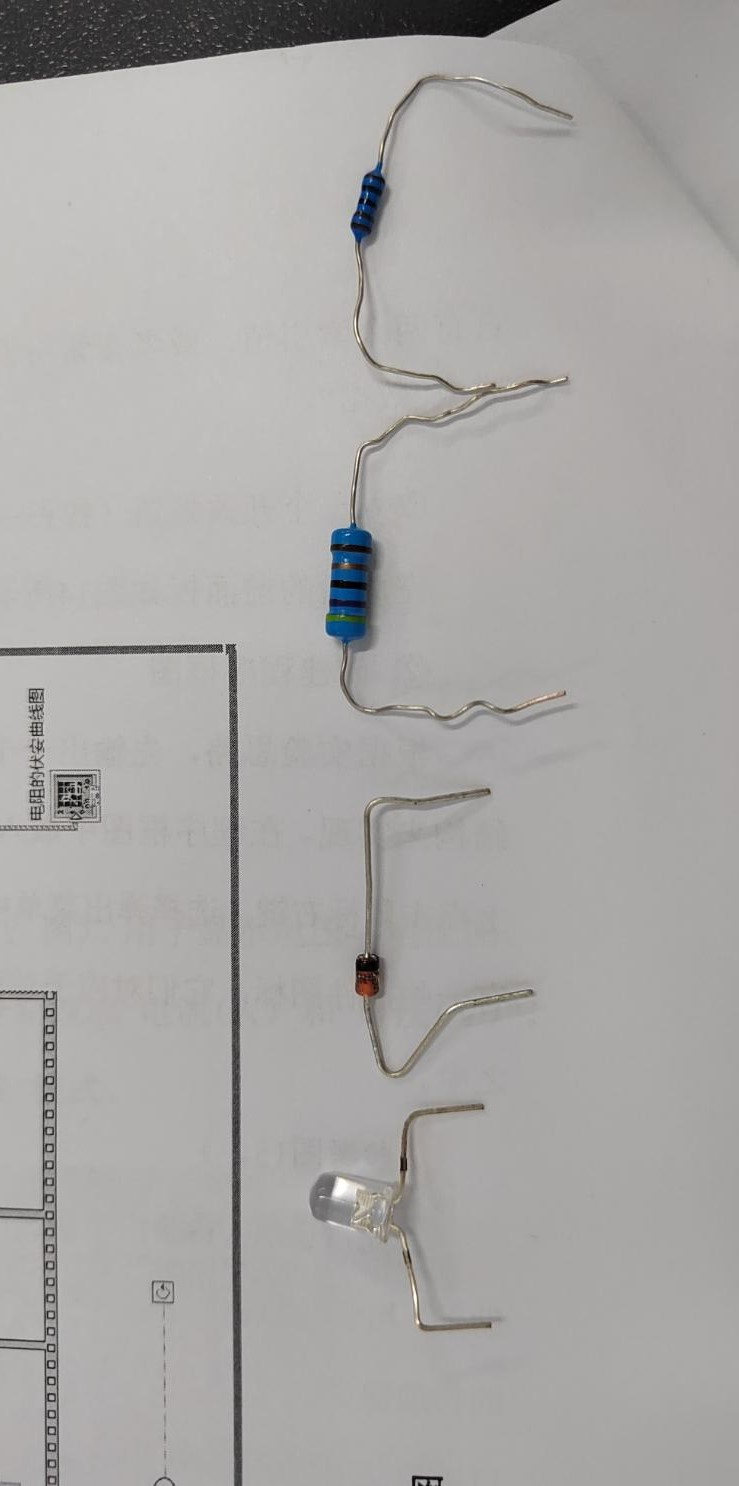
\includegraphics[height=250pt]{assets/附录/IMG_20241015_164842.jpg}
    \end{subfigure}
\end{figure}

\begin{figure}[H]\centering
    \begin{subfigure}[b]{0.5\columnwidth}\centering
        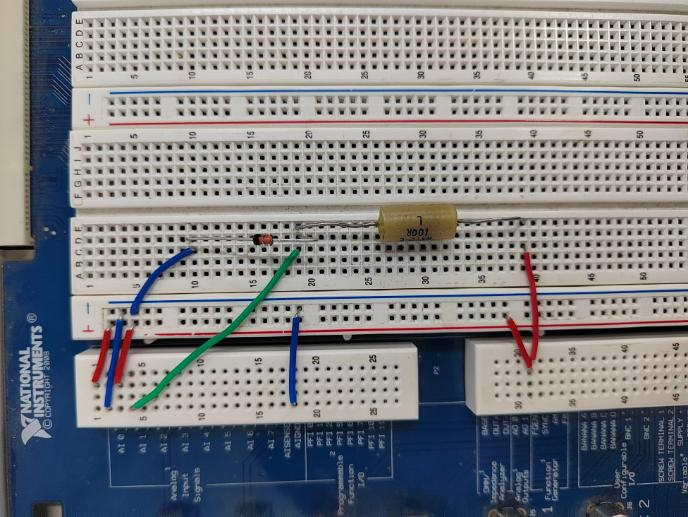
\includegraphics[height=170pt]{assets/附录/IMG_20241015_163203.jpg}
    \end{subfigure}\hfill
    \begin{subfigure}[b]{0.5\columnwidth}\centering
        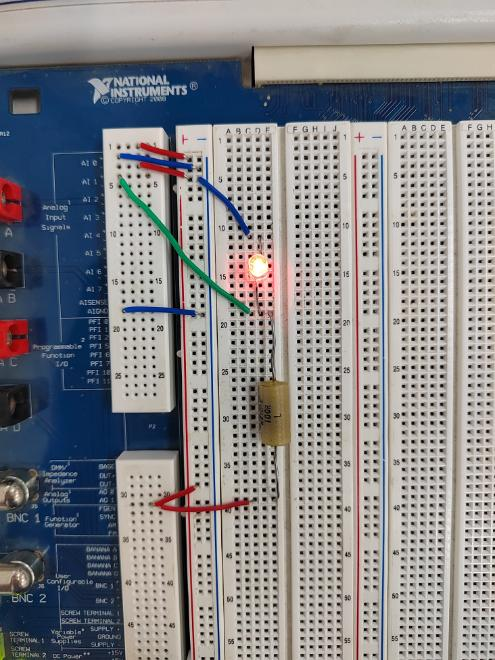
\includegraphics[width=170pt, angle=90]{assets/附录/IMG_20241015_163454.jpg}
    \end{subfigure}
\end{figure}

\begin{figure}[H]\centering
    \begin{subfigure}[b]{0.5\columnwidth}\centering
        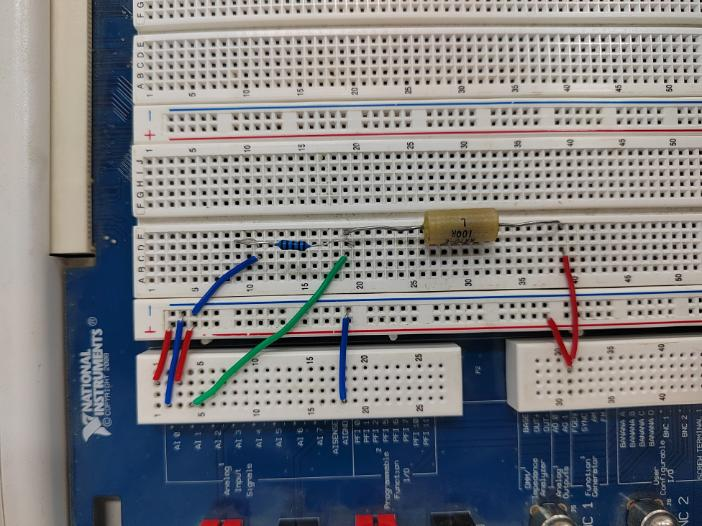
\includegraphics[height=170pt]{assets/附录/IMG_20241015_164039.jpg}
    \end{subfigure}\hfill
    \begin{subfigure}[b]{0.5\columnwidth}\centering
        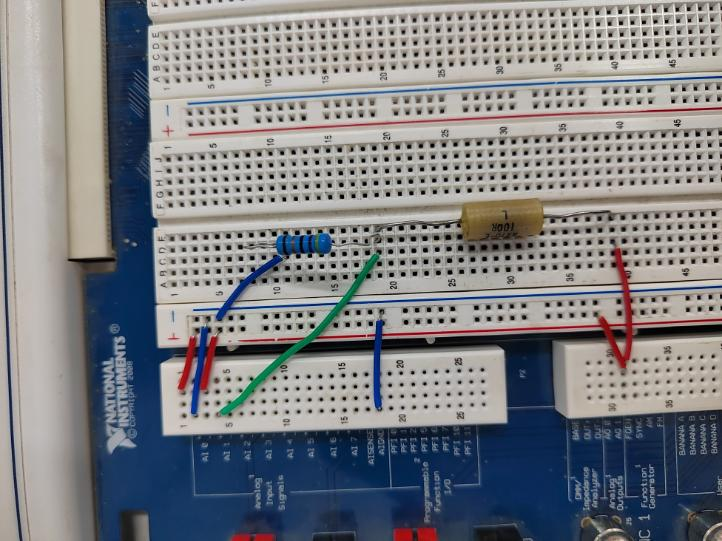
\includegraphics[height=170pt]{assets/附录/IMG_20241015_164436.jpg}
    \end{subfigure}
\end{figure}





\end{document}

% VScode 常用快捷键:

% F2:                       变量重命名
% Ctrl + Enter:             行中换行
% Alt + up/down:            上下移行
% 鼠标中键 + 移动:           快速多光标
% Shift + Alt + up/down:    上下复制
% Ctrl + left/right:        左右跳单词
% Ctrl + Backspace/Delete:  左右删单词    
% Shift + Delete:           删除此行
% Ctrl + J:                 打开 VScode 下栏(输出栏)
% Ctrl + B:                 打开 VScode 左栏(目录栏)
% Ctrl + `:                 打开 VScode 终端栏
% Ctrl + 0:                 定位文件
% Ctrl + Tab:               切换已打开的文件(切标签)
% Ctrl + Shift + P:         打开全局命令(设置)

% Latex 常用快捷键:

% Ctrl + Alt + J:           由代码定位到PDF


